\documentclass[12pt,a4paper]{report}
\usepackage{amsmath}    % Advanced Mathematics
\usepackage{graphicx}   % Include PostScript figures
\usepackage{makeidx}    % Makeindex
\usepackage{a4wide}
\usepackage[round]{natbib}     % Bibliography



\makeindex

\title{VertEgg -- A toolbox for simulation of vertical distributions 
of fish eggs \\ Version 1.0}

\author{Bj{\o}rn {\AA}dlandsvik \\
        Institute of Marine Research \\
        P.O. Box 1870, Nordnes \\
        N-5024 Bergen \\
        Norway \\
        E-mail: bjorn@imr.no}

% Inkluder mattemakroer og enheter
\newcommand{\be}{\begin{equation}}
\newcommand{\ee}{\end{equation}}
\newcommand{\bel}[1]{\begin{equation}\label{#1}}
\newcommand{\Pd}[2]{\frac{\partial #1}{\partial #2}}
\newcommand{\Od}[2]{\frac{d#1}{d#2}}
\newcommand{\Pdp}[2]{\frac{\partial }{\partial #2}(#1)}
\newcommand{\Odp}[2]{\frac{d}{d#2}(#1)}
\newcommand{\Dt}{\Delta t}
\newcommand{\Dx}{\Delta x}
\newcommand{\Dy}{\Delta y}
\newcommand{\Dz}{\Delta z}
\newcommand{\Lik}[1]{(\ref{#1})}
\newcommand{\pref}[1]{(\ref{#1})}
\newcommand{\Fig}[1]{Figure \ref{#1}}
\newcommand{\dt}{\delta t}
\newcommand{\Grad}{\nabla}
\newcommand{\Div}{\nabla\cdot}
\newcommand{\dps}{\displaystyle}
\newcommand{\Pdd}[2]{ \frac{ \partial^{2} {#1} }{ \partial {#2}^{2} } }
\newcommand{\Ds}{\Delta s}
\newcommand{\pddx}{\frac{\partial}{\partial x}}
%
% Bidrag fra Bj\o rn
% 
% Generelle mattemakroer
%
\newcommand{\pddt}{\frac{\partial}{\partial t}} 
\newcommand{\pddz}{\frac{\partial}{\partial z}} 
\newcommand{\half}{\ensuremath{\frac{1}{2}}}
\newcommand{\abs}[1]{|#1|}
%
% Nyttige enheter; 
%    - mattemode ingen problemer.
%    - tekstmode bruk: ... tall\enhet\ neste ord ...
%    System: sq = ^2, cu = ^3, p = "per" d.v.s. /
%
\newcommand{\s}{\ensuremath{\, \mbox{s}}}                     % s
\newcommand{\m}{\ensuremath{\, \mbox{m}}}                     % m
\newcommand{\mm}{\ensuremath{\, \mbox{mm}}}                   % mm
\newcommand{\mps}{\ensuremath{\, \mbox{m} \mbox{s}^{-1}}}     % m/s
\newcommand{\cmps}{\ensuremath{\, \mbox{cm} \mbox{s}^{-1}}}   % cm/s
%\newcommand{\mmps}{\ensuremath{\, \mbox{mm} \mbox{s}^{-1}}}   % mm/s
\newcommand{\mmps}{\ensuremath{\, \mbox{mm} / \mbox{s}}}   % mm/s
\newcommand{\sqmps}{\ensuremath{\, \mbox{m}^2 \mbox{s}^{-1}}} % m^2/s
\newcommand{\kgpcum}{\ensuremath{\, \mbox{kg} \mbox{m}^{-3}}} % kg/m^3
\newcommand{\Sv}{\ensuremath{\,}\mbox{Sv}}           % Sv
\newcommand{\degC}{\ensuremath{^\circ}\mbox{C}}      % grader Celcius
\renewcommand{\deg}{\ensuremath{^\circ}}             % grader
%\renewcommand{\min}{\ensuremath{^\prime}}            % minutter




%\includeonly{appendix}


\pagestyle{headings}

\setcounter{tocdepth}{3}


\renewcommand{\phi}{\varphi}

% Mer spesielle mattemakroer
%\newcommand{\Fconv}{\ensuremath{F^{\mathit{conv}}}}  % Convective flux
%\newcommand{\Fdiff}{\ensuremath{F^{\mathit{diff}}}}  % Diffusive flux
\newcommand{\Fconv}{\ensuremath{F^{\mathrm{conv}}}}  % Convective flux
\newcommand{\Fdiff}{\ensuremath{F^{\mathrm{diff}}}}  % Diffusive flux
\newcommand{\Qspawn}{\ensuremath{Q^{\mathrm{spawn}}}}  %
\newcommand{\Qloss}{\ensuremath{Q^{\mathrm{loss}}}}  % 
\newcommand{\Pcell}{\ensuremath{P^{\mathrm{cell}}}}
\newcommand{\e}{\ensuremath{\mathrm{e}}}
\renewcommand{\i}{\ensuremath{\mathrm{i}}}

\newcommand{\Vint}{\int_{-H}^0}        % Vertical integral

% Nyttige enheter
%\newcommand{\parm}{\text{$\mbox{particles} / \text{m}^{3}$}\ }


% Ymse
\newcommand{\shortcite}[1]{(\citeyear{#1})}
%\bibpunct{(}{)}{;}{a}{,}{,}


% Fontskifte for EDB-tekniske utrykk 
%\newcommand{\edb}[1]{{\texttt{#1}}}
\newcommand{\edb}[1]{{\mbox{\texttt{#1}}}}
% EDB-teknisk + index
\newcommand{\edbi}[1]{{\mbox{\texttt{#1}}}\index{#1@\texttt{#1}}}
\newcommand{\indextt}[1]{\index{#1@\texttt{#1}}}
% Emphasis + index
\newcommand{\emphi}[1]{\emph{#1}\index{#1}}


% Milj� for skriving av code fragmenter
%\newenvironment{source}{\begin{verbatim}}{\end{verbatim}}
\newenvironment{source}
   {\begin{list}{}{\setlength{\leftmargin}{30pt}} \ttfamily \item[]}
   {\end{list}}   

%%%% Beskrivelser av verkt�y
% Headerlinjen
\newcommand{\thead}[2]%
   {\vspace{4mm}\underline{{\bfseries\large #1} -- #2}%
    \index{#1@\texttt{#1}|emph}}
% Milj�
\newcommand{\tdesclabel}[1]{\mbox{\textsf{#1:}}\hfil}
\newenvironment{tdesc}
  {\begin{list}{}%
     {\renewcommand{\makelabel}{\tdesclabel}%
      \setlength{\labelwidth}{13mm}%
      \setlength{\leftmargin}{\labelsep}%
      \addtolength{\leftmargin}{13mm}%
     }%
  }%
  {\end{list}}
% Tabbing av argumentlister
\newenvironment{vartab}%
   {\begin{tabbing}%
 Temperature \= : \= Vertically integrated concentration \= [deg C] \kill}%
   {\end{tabbing}}


\renewcommand{\topfraction}{0.8}
\renewcommand{\bottomfraction}{0.6}
\renewcommand{\textfraction}{0.1}



%%%%%%%%%%%%%%%%%%%%%%%%%%%%%%%%%%%%%%%%%%%%%%%%%
     

\begin{document}


\maketitle

\tableofcontents 

\clearpage
\addcontentsline{toc}{chapter}{Introduction}

\chapter*{Introduction}

The vertical distribution of fish eggs in a water column is determined
by the buoyant forcing and turbulent mixing.  A model of the steady
state distribution has been developed by Sundby \shortcite{sund83}.
Westg{\aa}rd \shortcite{west89} developed two numerical models for the time
evolution of the concentration. These models are written in FORTRAN
and use the GPGS library for graphics.

The commercial software system Matlab and the free alternative Octave
provide interactive command-line environments for numerical computations
and visualisation.  VertEgg is a toolbox for scientific work on
vertical egg distributions in these environments. It contains tools for
analysing observed distributions and performing numerical simulations
including pre- and post-processing of the results. VertEgg is
\emph{not} a finished application, the tools are intended to be used
interactively or sewed together by the user to make the application
that solves her problem. This approach should give the competent user a
powerful and flexible environment for research on vertical distributions.

The author believes strongly in learning by problem solving and
examples. Therefore the main part of the manual is the example chapter.
The examples ranges from simple illustrations of the functions in the
toolbox, by verification and sensitivity studies to a ready-to-run
egg-distribution model complete with file I/O.
These examples are also available online as \emph{scripts}, programs in
the internal programming language of the packages. The recommended way
to make small applications is to take the closest example script and
try out modifications.

The first two chapters give an introduction to the theory of vertical
egg distributions and the numerical method used. The manual also has a
chapter containing the reference manual, a systematic description of the
tools provided in VertEgg.

% Ta noe om tilgjengelighet, copyright ??



%
%  Teori.tex
%  Part of VertEgg documentation
%

\chapter{Theory of Vertical Egg Distributions}

\section{The Equations}\label{sec:equations}


Neglecting horizontal processes, the evolution of the vertical
distribution
of a class of fish eggs is governed by a simple \emph{conservation}
principle\index{conservation principle}

\begin{equation}\label{eq:consprin}
\begin{split}
  \text{The change}\ & \text{in the number of eggs between two depth levels} \\
  & = \text{the number of eggs entering at the lower level} \\
  & - \text{the number of eggs leaving at the upper level} \\
  & + \text{the number of eggs spawned} \\
  & - \text{the number of eggs that hatched or died}
\end{split}
\end{equation}

To put this in a more mathematical formulation, let the variable
$z$ denote depth and $t$ time. The $z$-axis is chosen to point
\emph{up}, that is $z = 0$ at the surface and negative values are
used in the water column. This choice is opposite from
\cite{sund83,sund91} and \cite{west89}. The present choice is
motivated by the most
common axis-convention in 3D hydrodynamic ocean modelling.

To make the theory more convenient mathematically, a
\emphi{continuum} approach is used, where the eggs are
replaced by a continuous egg \emphi{concentration}.  Let $\phi =
\phi(z,t)$ denote this egg concentration at depth $z$ and time
$t$. Let $F = F(z,t)$ be the upwards egg \emphi{flux}, i.e.\ the net
number of eggs passing upwards per time unit at depth $z$ and time
$t$. Similarly, let $Q = Q(z,t)$ denote the \emphi{source term}, the
number of eggs spawned minus the numbers that hatched or died per
depth and time unit at depth $z$ and time $t$.  The source term can
also be used to take care of other processes, such as loss of eggs by
horizontal advection.

The conservation principle \ref{eq:consprin} can then be formulated
in \emphi{integral form}
\begin{equation}\label{eq:intlaw}
\int_{z_1}^{z_2} \!\phi(z,t_2)\,dz - \int_{z_1}^{z_2}\!\phi(z,t_1)\,dz
   = \int_{t_1}^{t_2} \!F(z_1,t)\,dt
   - \int_{t_1}^{t_2} \!F(z_2,t)\,dt
   + \int_{t_1}^{t_2}\!\int_{z_1}^{z_2} \!Q(z,t)\,dzdt
\end{equation}
Mathematically this can be reformulated in mixed form, differential in time
and integral in space
\begin{equation}\label{eq:diffintlaw}
  \pddt \left( \int_{z_1}^{z_2} \!\phi(z,t)\,dz \right) =
  F({z_1},t) - F({z_2},t) + \int_{z_1}^{z_2}\!Q(z,t)\,dz
  \quad \mbox{for} \ -H \le {z_1} < {z_2} \le 0 .
\end{equation}
or in pure \emph{differential} form\index{differential form}
\begin{equation}\label{eq:difflaw}
  \Pd{\phi}{t} =  - \Pd{F}{z} + Q
\end{equation}

The flux is decomposed in two parts, the \emphi{convective flux} and the
\emphi{diffusive flux}.  The convection is due to the terminal buoyant
velocity $w = w(z,t)$ of the egg which is computed by the density
difference from the surroundings  and the egg size as described in section
\ref{sec:velocity}. The formulation is simply,
\begin{equation}\label{eq:convflux}
  \Fconv = w \phi .
\end{equation}
The diffusion is caused by turbulent mixing and is modelled by
Fick's law\index{Fick's law} using the vertical eddy diffusion
\index{eddy diffusion} $K = K(z,t)$,
\begin{equation}\label{eq:fick}
  \Fdiff = - K \frac{\partial \phi}{\partial z} .
\end{equation}

Often the source term $Q$ can be separated in a
\emph{spawning}\index{spawning term} or \emph{production}
term\index{production term} independent of the egg concentration
\begin{equation}\label{eq:spawn}
  \Qspawn = P
\end{equation}
and a \emph{mortality}\index{mortality term} or \emph{loss}
term\index{loss term} depending on the concentration
\begin{equation}\label{eq:loss}
  \Qloss = - \alpha \phi
\end{equation}
Using this the differential conservation law (\ref{eq:difflaw})
becomes
\bel{eq:difflawfull}
\Pd{\phi}{t} =  - \pddz (w \phi) + \pddz (K \Pd{\phi}{z}) + P - \alpha \phi
\end{equation}
This parabolic partial differential equations is
called the \emph{convection-diffusion}\index{convection-diffusion equation}
or \emph{transport} equation\index{transport equation}.

The boundary conditions\index{boundary conditions} are simply no flux
across the surface and bottom,
\bel{eq:boundcond}
  F(0,t) = F(-H,t) = 0,
\end{equation}
and the initial condition is given by
\bel{eq:initcond}
  \phi(z,0) = \phi_0(z),  \quad -H \le z \le 0.
\end{equation}

\section{Solutions of the equations}

Under simplified circumstances the equations in section~\ref{sec:equations}
can be solved analytically. This section examines some of these solutions.

\subsection{Vertical integrated equation}\label{sec:vertint}

Let $\Phi$ denote the total concentration, $\Phi = \Vint \phi dz$.
Take the vertical integral of equation~(\ref{eq:difflawfull}) and
use the boundary conditions (\ref{eq:boundcond}) gives
\be
\Od{\Phi}{t} = P^{tot} - \Vint \!\alpha \phi \, dz
\end{equation}
where $P^{tot} = \Vint P dz$ is the total spawning contribution.
Without any source terms the total concentration $\Phi$ is constant.
To reach a steady state solution with spawning, the loss term $\alpha$
must be nonzero.


If $\alpha$ is a positive
constant, the solution to the equation above is
\be
  \Phi(t) = \e^{-\alpha t} \Phi(0)
         + (1 - \e^{-\alpha t})  \frac{P^{tot}}{\alpha}
\end{equation}
with steady state solution $\Phi = P^{tot}/\alpha$.
If $\alpha = 0$ the solution is simply
\be
  \Phi(t) = \Phi(0) + t P^{tot} .
\end{equation}


\subsection{Stationary solution}\index{stationary solution}

A stationary solution solves the conservation law
\pref{eq:difflaw} without the time derivative
\begin{equation}\label{eq:stateq}
  \Od{F}{z} = Q
\end{equation}
with boundary conditions $F(0) = F(-H) = 0$ given by \pref{eq:boundcond}.
The condition for the existence of this solution is that the total
source term vanishes,
\begin{equation}
  Q^{tot} = \Vint \!Q \, dz= 0
\end{equation}
the flux function is then given by integrating \pref{eq:stateq}
\begin{equation}
  F(z) = \int_{-H}^z \! Q(s) \, ds = - \int_z^0 \! Q(s) \, ds .
\end{equation}

Without source term the expression above reduces to $F = 0$, i.e.\ the
net flux is zero everywhere. This simply says that in a steady state
convection is balanced by diffusion
\bel{eq:sstate}
  w \phi - K \Pd{\phi}{z} = 0 .
\end{equation}
This is an ordinary differential equation for $\phi(z)$.
The boundary conditions \pref{eq:boundcond} does not contain more information.
A unique solution can nevertheless be singled out by the
integral condition
\begin{equation}\label{eq:intcond}
  \Vint \!\phi(z)\,dz = \Phi .
\end{equation}
In other words, among all the solutions of (\ref{eq:sstate})
choose the one with correct vertically integrated concentration.

To simplify the notation put $m = w / K$ and let $M(z) = - \int_z^0 m(s)
ds$. Then the stationary solution is
\begin{equation}\label{eq:sstatesol}
  \phi(z) = \frac{\Phi}{\int_{-H}^0 \e^{M(s)} ds} \e^{M(z)} .
\end{equation}

\subsubsection{Constant coefficients}

The case with constant coefficients was studied by Sundby
\shortcite{sund83}.  In this case $M(z) = m z$ and the solution is a
truncated exponential distribution,
\begin{equation}\label{eq:eggsact}
  \phi_m(z) = \Phi \frac{m}{1 - \e^{-mH}} \e^{mz} .
\end{equation}
In the toolbox, this solution is computed by the function \edbi{eggsact}.
This solution has the following symmetry between ascending and
descending velocity,
\begin{equation}\label{eq:symmetry}
  \phi_{-m}(z) = \phi_m(-H-z)
\end{equation}

With large depth and/or high ascending velocity  the
effect of the bottom may be neglected. In this case the distribution
is well approximated by an exponential distribution \index{exponential
distribution} with parameter $\lambda = 1 / m$, that is
\begin{equation}
  \phi_m(z) \approx \Phi m \e^{mz}, \quad \text{for $mH \gg 1$} .
\end{equation}


For positive values of $m$ the following series development from
\citep{sund83} is valid
\begin{equation}
  \phi_m(z) = \Phi m \e^{mz} \sum_{j = 0}^{\infty} \e^{-jmH}, \quad m > 0 .
\end{equation}
The zero-th term of this expansion is the exponential distribution above.
For negative values of $m$ the symmetry relation (\ref{eq:symmetry})
can be used,
\begin{equation}
  \phi_m(z) = - \Phi m \e^{mz} \sum_{j = 1}^{\infty} \e^{jmH}, \quad m < 0 .
\end{equation}

To compute the mean and variance of the distribution the constant
factor $\Phi$ can be dropped. The moment generating function is then
\begin{equation}\label{eq:momgen}
  \psi(t) = \int_{-H}^0 \frac{m}{1 - \e^{-mH}} \e^{(m+t)z} dz
          = \frac{m}{1 - \e^{-mH}} \frac{1 - \e^{-(m+t)H}}{m+t}.
\end{equation}
Differentiating $\psi$ gives the moments of the distribution.
The mean depth is given by
\begin{equation}\label{eq:eggsactmean}
  \mu = \psi'(0) = - \frac{1}{m} + \frac{H}{\e^{mH} - 1}
\end{equation}
The function $\mu = \mu(m)$ with $H = 100\m$ is plotted in
figure~\ref{fig:mdepth}.  The variance is
\begin{equation}\label{eq:eggsactvar}
       \psi''(0) - \mu^2
      = \frac{2 - \e^{-mH}(m^2 H^2 + 2 m H + 2)}{m^2 ( 1 - \e^{-mH})} - \mu^2
\end{equation}


\begin{figure}
\begin{center}
\includegraphics[height=6cm]{mdepth}
\end{center}
\caption{Mean depth $\mu$ as a function of $m$}\label{fig:mdepth}
\end{figure}

\subsubsection{Piecewise constant coefficients}

The solution (\ref{eq:eggsact}) can easily be extended to a piecewise
constant $m$.
Let $0 = z_0 > \cdots > z_m = -H$ be a partition of the water column
with $m(z) = m_i$ on the interval $I_i = (z_i, z_{i-1})$.
Then the stationary solution restricted to the interval $I_i$ is
given as
\begin{equation}\label{eq:pwconst}
  \phi(z) = C_i \e^{m_i z}, \quad \mbox{for} \ z_i < z < z_{i-1}
\end{equation}
The $C_i$-s are determined by continuity
of the solution
\begin{equation}
  C_i \e^{m_i z_i} = C_{i+1} \e^{m_{i+1} z_i}, \quad  i = 1, \ldots, m-1
\end{equation}
and the integral condition~(\ref{eq:intcond})
\begin{equation}
   \sum_{i = 1}^m C_i \int_{z_i}^{z_{i-1}} \e^{m_i z} dz
   = \sum_{i = 1}^m C_i \frac{\e^{m_i z_{i-1}} - \e^{m_i z_i}}{m_i}
   = \Phi .
\end{equation}
This method is used in the function \edbi{sstate} to approximate the
general steady state solution. More details of the implementation is
given in section~\ref{sec:statprob}.


\subsubsection{Linear coefficients}

In Sundby \shortcite{sund91} the solution is derived for $m$ linear.
Let $m$ be given as $m(z) = a (z-z_0)$. Then $M(z) =
\half a ((z - z_0)^2 - z_0^2)$. Taking the last term into the
constant $C$, the solution becomes
\begin{equation}
  \phi(z) = C \e^{\half a (z - z_0)^2} .
\end{equation}
Bathypelagic eggs are neutral buoyant at $z = z_0$, raising if deeper
and sinking if higher in the water column. In this case the coefficient
$a$ is negative and the concentration has a normal distribution about $z =
z_0$ with variance $\sigma^2 = {1 / |a|}$.

%In a sample of eggs the diameters and buoyancies differ from egg to egg.
%A more realistic model of the stationary situation will therefore be to
%use a distribution of the $m$-values. This task was studied by Sundby (1983).
%...


\subsubsection{Stationary solution with source terms}

With source terms, the steady state equation is
\begin{equation}\label{eq:srcsstate}
  0 = - \pddz (w \phi) + \pddz (K \Pd{\phi}{z}) + P - \alpha \phi .
\end{equation}
This is a general second order ordinary
differential equation. With constant coefficients the equation becomes
\begin{equation}\label{eq:srcsacteq}
  K \phi'' - w \phi' - \alpha \phi = - P
\end{equation}
and the no flux boundary conditions are
\begin{equation}
  K \phi' - w \phi, \quad z = 0, z = -H .
\end{equation}
The solution can be written
\bel{eq:srssact}
  \phi(z) = A \e^{az} - B \e^{-bz} + \frac{P}{\alpha}
\end{equation}
with
\begin{align}
  a & = \frac{1}{2K} ( \sqrt{w^2 + 4 \alpha K} + w ) \\
  b & = \frac{1}{2K} ( \sqrt{w^2 + 4 \alpha K} - w ) \\
  A & = \frac{w P}{\alpha b K} \frac{1-\e^{-b H}}{1-\e^{-(a+b)H}} \\
  B & = \frac{w P}{\alpha a K} \e^{-b H} \frac{1-\e^{-a H}}{1-\e^{-(a+b)H}} .
\end{align}

This function is computed in the toolbox by the function \edbi{srcsact}.
The signs are chosen such that positive velocity $w$ makes all terms
positive. For negative velocities a symmetry property
similar to equation~(\ref{eq:symmetry})
can be used, if
$\phi(z)$ is a solution to equation (\ref{eq:srcsacteq}) and boundary
conditions (\ref{eq:boundcond}) then $\phi(-H-z)$ is a solution the
same equation and boundary conditions with the opposite sign on $w$.
In other words,
\begin{equation}
  \phi_{-w}(z) = \phi_w(-H-z) .
\end{equation}


\section{The Terminal Egg Velocity}\label{sec:velocity}
\index{egg velocity}\index{terminal velocity}

An egg in sea water will reach its terminal velocity $w$, where the
buoyant forcing balances the frictional drag. This velocity is a
function of the difference $\Delta \rho = \rho - \rho_e$ between the
density of the water and the egg, the egg diameter $d$, the
acceleration $g$ due to gravity and the molecular
viscosity\index{molecular viscosity}. Here the \emph{dynamic}
molecular viscosity\index{dynamic viscosity} $\mu$ is used.

The situation is characterised by the non-dimensional \emphi{Reynolds
number},
\begin{equation}
  Re = \frac{\rho d w}{\mu}
\end{equation}
For low values, $Re < 0.5$, the terminal velocity is given by
\emphi{Stokes' formula}
\begin{equation}\label{eq:stokes}
  w = \frac{1}{18} \frac{g d^2 \Delta \rho}{\mu} .
\end{equation}
This formula was obtained by Stokes \shortcite{stok1851}. The
derivation of the formula is given in almost any textbook on
fluid dynamics, for instance \citep{yih77}.


Combining these equations, one obtains an expression for $D$, the maximum
diameter for which Stokes' velocity applies,
\begin{equation}
  D^3 = \frac{9 \mu^2}{\rho g \Delta \rho}
\end{equation}


In the intermediate region $0.5 < Re < 5$, Dallavalle (1948) gave an
empirical formula\index{Dallavalle's formula}
\begin{equation}\label{eq:dallavalle}
  w = K_I (d - \zeta D) \Delta \rho^{2/3} \mu^{-1/3}
\end{equation}
where $\zeta = 0.4$ for a sphere. The coefficient $K_I$ is determined
by the requirement that both formulas should give the same answer for
$Re = 0.5$ or equivalently $d = D$.
This gives
\begin{equation}
  K_I = \frac{5}{54} 9^{1/3} g^{2/3} \rho^{-1/3}
         = 0.0875 \text{kg}^{-1/3} \,
             \text{m}^{5/3} \text{s}^{-4/3} .
\end{equation}

The formulas above are implemented as the function \edbi{eggvel} in
the VertEgg toolbox. The buoyancy of a fish egg is often given as the
salinity $S_e$ where the egg is neutrally buoyant. The function
\edbi{eggvelst} computes the terminal velocity in this case.


To compute the egg velocity the density, $\rho$ of water is needed.
In the toolbox only density at surface pressure is presently
available.  This is computed by the function \edbi{dens0} by the
UNESCO formula \citep{UNES81}.  The function \edbi{sw\_dens} in the
SEAWATER toolbox\index{SEAWATER} \citep{morg94} has implemented the
full UNESCO equation of state.

The dynamic molecular
viscosity\index{viscosity!molecular}\index{viscosity!dynamic} $\mu$ of
sea water is tabulated in table \ref{tab:molvisc} taken from Sverdrup
\emph{et al.}
\shortcite{sver52}. The values decrease  with temperature and increase
slowly with salinity. The dependence on pressure is insignificant, and is
neglected here.

\begin{table}[h]
\begin{center}
\begin{tabular}{|c|c|c|c|c|c|c|c|}
\hline\hline
Salinity   & \multicolumn{7}{c|}{Temperature [\deg C]} \\
\cline{2-8}
[psu] & 0 & 5 & 10 & 15 & 20 & 25 & 30 \\
\hline
 0 & 1.79 &  1.52 & 1.31 & 1.14 & 1.01 & 0.89 & 0.80 \\
10 & 1.82 &  1.55 & 1.34 & 1.17 & 1.03 & 0.91 & 0.82 \\
20 & 1.85 &  1.58 & 1.36 & 1.19 & 1.05 & 0.93 & 0.84 \\
30 & 1.88 &  1.60 & 1.38 & 1.21 & 1.07 & 0.95 & 0.86 \\
35 & 1.89 &  1.61 & 1.39 & 1.22 & 1.09 & 0.96 & 0.87 \\
\hline
\end{tabular}
\end{center}
 \caption{Dynamic molecular viscosity of sea water
  with unit $10^{-3} \,\text{kgm}^{-1}\text{s}^{-1}$}
  \label{tab:molvisc}
\end{table}


Using linear least squares regression the table is approximated by the
following function where $T$ is the temperature in \deg C and $S$ is
the salinity in psu.
\begin{equation}\label{eq:molvisc}
  \mu = 10^{-3} \, (1.7915 - 0.0538 \, T + 0.007 \, T^2 - 0.0023 \, S )
            \:   \text{kgm}^{-1}\text{s}^{-1} ,
\end{equation}
This reproduces table \ref{tab:molvisc} with an absolute error less
than $2 \times 10^{-5}\, \text{kgm}^{-1}\text{s}^{-1}$ and a relative
error of 1.7 \%. This is good enough to compute egg velocities where
the uncertainty in the other variables are larger.  This formula is
implemented by the function
\edbi{molvisc} in the toolbox. Riley and Skirrow \shortcite{rile75}
give a more precise formula which requires more computational effort.


% numerikk.tex
% Part of VertEgg documentation
%


\chapter{Numerical Methods}



The numerical solutions are computed on a fixed equidistant grid.  The
number of grid cells is denoted $N$ and the cell height is $\Delta
z$. The grid is staggered as shown in fig.~\ref{fig:grid}.  The
$z$-axis points upwards.
 
The cell interfaces, the \emph{flux points}\index{flux points}, are 
\begin{equation}\label{eq:flushpt}
  z_i = (1-i) \Dz \quad \text{for} \quad i = 1, \dots, N+1 .
\end{equation}
The cell centers, the \emph{concentration points}\index{concentration
points} or the \emphi{egg points}, are
\begin{equation}\label{eq:eggpt}
  \bar{z}_i = \frac{z_i + z_{i+1}}{2} = (\half-i) \Dz
            \quad \text{for} \quad i = 1, \dots, N .
\end{equation}

\begin{figure}[h]
\begin{center}
\setlength{\unitlength}{1mm}
\begin{picture}(65,20)
  \multiput(10.0, 8.5)(20,0){3}{\line(0, 1){3}}
  \put(20.0,10.0){\makebox(0,0){$\times$}}
  \put(40.0,10.0){\makebox(0,0){$\times$}}
  \put(10.0, 6.0){\makebox(0,0){$z_{i+1}$}}
  \put(30.0, 6.0){\makebox(0,0){$z_{i}$}}
  \put(50.0, 6.0){\makebox(0,0){$z_{i-1}$}}
  \put(20.0, 6.0){\makebox(0,0){$\bar{z}_{i}$}}
  \put(40.0, 6.0){\makebox(0,0){$\bar{z}_{i-1}$}}
  \put(10.0,14.0){\makebox(0,0){$F_{i+1}$}}
  \put(30.0,14.0){\makebox(0,0){$F_{i}$}}
  \put(50.0,14.0){\makebox(0,0){$F_{i-1}$}}
  \put(20.0,14.0){\makebox(0,0){$\phi_{i}$}}
  \put(40.0,14.0){\makebox(0,0){$\phi_{i-1}$}}
  \put(0,10){\vector(1,0){60}}
\end{picture}
\end{center}
\caption{Horizontal view of the vertical grid}\label{fig:grid}
\end{figure}

The variables are discretized in the following ways. The egg
concentration $\phi_i$ represents the mean concentration in
cell $i$, that is
\begin{equation}\label{eq:cellav}
  \phi_i \Dz = \int_{z_{i+1}}^{z_i} \!\phi(z)\,dz, 
                 \quad i = 1, \dots ,N .
\end{equation}
The $\phi_i$ values may be considered living on the egg points
$\bar{z}_i$ as in fig.~\ref{fig:grid}. As the flux values are computed
from the vertical velocity and the eddy diffusivity,
$F_i$, $w_i$ and $K_i$ are taken as point values on the flux points
$z_i$ for $i = 1, \dots, N+1$. The source terms $P_i$ and $\alpha_i$
are cell averages and live on the egg points.


\section{The Transient Problem}\label{sec:numtrans}

The numerical solution of the convection-diffusion
equation~(\ref{eq:difflaw}) are covered by several authors.  A classic
source is Roache \shortcite{roac72}. A newer source is chapter 9 in
the book by Fletcher \shortcite{flet91}. Recently a whole book, edited
by Vreugdenhil and Koren \shortcite{vreu93}, has been devoted to this
equation.  For conservative methods, as will be used here, the book by
LeVeque \shortcite{leve92} is also recommended.

For our problem, convection and diffusion of concentration of fish
eggs, some properties of the numerical method is important.  Fish eggs
are usually found in a subrange of the water column with values close
to zero outside this range. And of course a real concentration do not
have negative values.  The method must therefore be
\emph{positive}, that is it must not create
any negative values.

In the absence of source and sink terms, eggs are not created or
destroyed. The vertical integrated concentration is therefore constant
in time as shown in section~\ref{sec:vertint}.  The numerical method
should have the same property, it should be \emph{mass
conserving}\index{mass conserving method}. 

Of course the numerical solution should be as close as possible to the
real solution. That is the \emph{accuracy} of the method should be
good. This concept includes low artificial diffusion and no or very
limited wiggles development.

A convection -- diffusion problem is characterised by the following
non-dimensional numbers, all defined at the interior flux points,
$z_i$ for $i = 2, \dots, N$.
\begin{align}
  & \text{Courant number}         & c_i & = w_i\frac{\Dt}{\Dz} \\
  & \text{Diffusive parameter}    & s_i & = K_i \frac{\Dt}{\Dz^2} \\
  & \text{Cell Peclet number}     & \Pcell_i & = 
       \frac{\abs{w_i} \Dz}{K} = \frac{\abs{c_i}}{s_i}
\end{align}
\index{Courant number}\index{diffusive parameter}\index{cell Peclet number}
If the coefficients $w$ and $K$
are constant, the subscripts are simply dropped.

For fish eggs, the terminal velocity is in the order of a couple of
millimetres per second. The velocity can be positive (\emph{pelagic}
eggs)\index{pelagic eggs}, negative (\emph{benthic})\index{benthic
eggs} or change sign some place in the water column
(\emph{mesopelagic})\index{mesopelagic eggs}. The vertical eddy
diffusion show a very large range of variation, from more than
$10^{-2}$ \sqmps\ in the upper mixing layer to $10^{-5} \sqmps$
in the pycnocline layer.  With a grid size of the
order of one meter, the Cell Peclet number $\Pcell$ take values from
$10^{-1}$ to $10^2$. This means that the process may be dominated by
diffusion in the upper layer and convection below.

The numerical methods considered here are \emph{finite difference} or
really \emph{finite volume} schemes given in \emph{conservation
form}\index{conservation form} (or \emph{flux
formulation}\index{flux formulation}).  These methods are
conceptually natural, working directly with the integral form of the
conservation law~(\ref{eq:intlaw}).  More precisely, the
equation~(\ref{eq:intlaw}) is approximated by
\begin{equation}\label{eq:numlaw}
  (\phi_i^{n+1} - \phi_i^n) \Dz = 
           (F_{i+1}^n - F_i^n) \Dt + Q_i^n \Dz \Dt ,
           \quad i = 2, \dots, N
\end{equation}
where the superscripts indicate the time step. 
The boundary conditions (\ref{eq:boundcond}) simply become
$F_1 = F_{N+1} = 0$. The various methods
differ in their estimation of the total flux function $F_i = \Fconv_i
+ \Fdiff_i$ and the source term $Q_i$.  One advantage of this flux
formulation is that mass conservation is automatically fulfilled, as
the fluxes cancel out during vertical integration.

Without source term the total concentration is conserved. Therefore
the local concentration values can not become arbitrary large, unless
there are negative values in some other cells. In other words,
positivity is a sufficient (but not necessary) condition for stability
of such schemes.

In the following several methods are described.  They are implemented in
the toolbox as \edbi{ftcs}, \edbi{lwendrof}, \edbi{upstream},
\edbi{posmet}, and \edbi{minlim} respectively. Their performance
will be studied in the example section~\ref{sec:sens}. Several methods
for the same problem causes a new problem, which method to choose. This
depends on the range of $\Pcell$ values in the problem. A general
advice is to try Lax-Wendroff first. This is an accurate and fast method
when applicable. If oscillations occur, go for the flux-limited
methods or use higher spatial resolution.  In both cases more computing
time is required. 



\subsection{Linear conservative schemes}\label{seq:linsch}

The linear conservative schemes considered here estimates the total 
flux function in the form 
\begin{equation}\label{eq:alphabeta}
  F_i = \alpha_i \phi_i + \beta_i \phi_{i-1} ,
\end{equation}
where the $\alpha_i$-s and $\beta_i$-s are independent of 
the $\phi_i$-s. Sometimes this will be used in non-dimensional form
\begin{equation}\label{eq:ab}
  F_i = \frac{\Dz}{\Dt} (a_i \phi_i + b_i \phi_{i-1}) .
\end{equation}
Some general theory for this kind of numerical schemes is presented
in Appendix~\ref{app:lincons}


\subsubsection{The FTCS scheme}\index{FTCS scheme}

The simplest scheme is often called FTCS (forward time central space)
after the differencing. This scheme is described for instance in
chapter 9.4 in \cite{flet91}. Here both flux
components are centred around $z = z_i$,
\begin{equation}
  \Fconv_i = w_i \frac{\phi_{i-1} + \phi_i}{2}
\end{equation}
\begin{equation}\label{eq:centdifflux}
  \Fdiff_i = - K_i \frac{\phi_{i-1} - \phi_i}{\Dz} .
\end{equation}
In the notation of equation (\ref{eq:alphabeta}) the method is given by
\begin{equation}
   \alpha_i = \frac{1}{2} w_i + \frac{K_i}{\Dz} , \quad 
   \beta_i  = \frac{1}{2} w_i - \frac{K_i}{\Dz} ,
\end{equation}
and non-dimensionalised by
\begin{equation}
   a_i = \frac{1}{2} c_i + s_i , \quad 
   b_i = \frac{1}{2} c_i - s_i .
\end{equation}

The following positivity condition for the FTCS scheme follows from
the general condition in Appendix~\ref{app:pos}.
\begin{gather}
     \abs{c_i} \le 2 s_i,  \quad i = 2, \dots, N \\
      s_2 \le 1 + \half c_2 \\
  s_i + s_{i+1} \le 1 + \half (c_i - c_{i+1}), \quad i = 2, \dots, N-1 \\ 
      s_N \le 1 - \half c_N
\end{gather}
The first condition can be restated as $\Pcell \le 2$.

With constant coefficients, the positivity conditions reduce to
\begin{equation}
  \abs{c} \le 2 s \le 1,
\end{equation}
which is stronger than the stability condition
\begin{equation}
  c^2 \le 2 s \le 1 .
\end{equation}

The numerical ``diffusion'' is negative, 
\begin{equation}
  K_{num} = - \half w^2 \Dt
\end{equation}
which is negligible if $c^2 \ll 2s$.

This method is implemented in the toolbox as the function \edbi{ftcs}.

\subsubsection{The Lax-Wendroff Scheme}\index{Lax-Wendroff scheme}

An alternative is the Lax-Wendroff scheme as analysed for instance in
\cite{vreu93b}. The scheme compensates for the negative numerical
``diffusion'' in FTCS.  The diffusive flux is still given by
equation~(\ref{eq:centdifflux}) but the convective flux is modified
\begin{equation}\label{eq:lwflux}
  \Fconv_i = w_i \frac{\phi_{i-1} + \phi_i}{2}
      - \half w_i^2 \frac{\Dt}{\Dz} 
       (\phi_{i-1} -\phi_i) .
\end{equation}
In the notation of equation (\ref{eq:alphabeta}) the Lax-Wendroff
method is given by
\begin{equation}
   \alpha_i = \frac{1}{2} w_i(1+w_i\frac{\Dt}{\Dz}) + \frac{K_i}{\Dz} , \quad 
   \beta_i  = \frac{1}{2} w_i(1-w_i\frac{\Dt}{\Dz}) - \frac{K_i}{\Dz} ,
\end{equation}
and non-dimensionalised by
\begin{equation}
   a_i = \frac{1}{2} c_i(1+c_i) + s_i , \quad 
   b_i = \frac{1}{2} c_i(1-c_i) - s_i .
\end{equation}

From Appendix~\ref{app:pos} the conditions for positivity are
\begin{gather}
     \abs{c_i} \le 2 s_i + c_i^2,  \quad i = 2, \dots, N \\
     s_i + s_{i+1} \le 1 + \half (c_i - c_{i+1}) - \half(c_i^2 + c_{i+1}^2),
               \quad i = 2, \dots, N-1.
\end{gather}
The first condition can be restated as 
\begin{equation}\label{eq:lwpcell}
    \Pcell \le \frac{2}{1-\abs{c_i}} .
\end{equation}

With constant coefficients, the positivity
conditions reduce to
\begin{equation}
 \abs{c} \le c^2 + 2 s \le 1,
\end{equation}
which is stronger than the stability condition
\begin{equation}
  c^2 + 2 s \le 1 .
\end{equation}

There is no second order numerical diffusion in the transient
solution.  Wiggles will not occur if the positivity
condition~(\ref{eq:lwpcell}) is fulfilled.
This method is implemented in the toolbox as the function \edbi{lwendrof}.

\subsubsection{The Upstream Scheme}\index{upstream scheme}

A non-centred alternative is the upstream method.  This is the method
used by West\-g{\aa}rd \shortcite{west89}.  The upstream scheme is
studied in all books on the subject.  The same diffusive flux
(\ref{eq:centdifflux}) is used but the convective flux is estimated on
the inflow side.
\begin{equation}\label{eq:usflux}
  \Fconv_i = w_i^+ \phi_i + w_i^- \phi_{i-1}
\end{equation}
where 
\begin{equation}
   x^+ = \half (x + |x|) = 
       \begin{cases}
          x& \text{if $x \ge 0$},\\
          0& \text{if $x  < 0$}.
       \end{cases}
\end{equation}
and $x^- = x - x^+$.
In the notation of equation (\ref{eq:alphabeta}) the method is given by
\begin{equation}
   \alpha_i =  w_i^+ + \frac{K_i}{\Dz} , \quad 
   \beta_i  =  w_i^- - \frac{K_i}{\Dz} ,
\end{equation}
and non-dimensionalised by
\begin{equation}
   a_i = c_i^+ + s_i , \quad 
   b_i = c_i^- - s_i .
\end{equation}

From Appendix~\ref{app:pos} the positivity condition is simply
\begin{equation}\label{eq:uspos}
  c_i^+ - c_{i+1}^- + s_i + s_{i+1} \le 1 .
\end{equation}
With constant coefficients this reduces to
\begin{equation}
  \abs{c} + 2 s \le 1 .
\end{equation}
which is also the stability condition.

The numerical diffusion in the upstream scheme may be quite large
\begin{equation}
  K_{num} = \half w \Dz (1-\abs{c})
\end{equation}
This is negligible if $K_{num} \ll K$, or equivalently
\begin{equation}
  \Pcell \ll \frac{2}{1 - \abs{c}} .
\end{equation}

The upstream scheme is implemented in the toolbox as the function
\edbi{upstream}.

\subsection{Nonlinear methods}\label{sec:nonlin}\index{non
linear method}

The Lax-Wendroff scheme is second order in space but may develop
wiggles and negative concentration values. The upstream method is
positive but may be too diffusive. These are fundamental problems with
linear schemes.  Several nonlinear schemes has been developed to
overcome these problems.  A general idea is to combine the
Lax-Wendroff and upstream methods to produce positive schemes with low
numerical diffusion. Overviews of such methods are given by LeVeque
\shortcite{leve92} and in the collection \citep{vreu93}.

Egg distribution problems are somewhat non-symmetrical. It is
important to have high accuracy near maxima where most of the eggs are
found. Local minima are less interesting and they occur more seldom in
the interior of the water column. For instance, with the steady state
solution (\ref{eq:sstatesol}) without source terms, a local minimum in
the interior can occur only in static instable situations when the egg
is lighter than the water above and heavier saline than the water
below.

The methods below are not total variation diminishing (TVD) as some of
the more advanced non-linear methods.  Instead of a finely tuned
linear combination, the schemes use simple on/off mechanisms to switch
between the Lax-Wendroff and upstream fluxes.  On the other hand, the
asymmetry above is exploited. The schemes have high accuracy at maxima
because the unmodified Lax-Wendroff flux is used in this situation.



\subsubsection{The positive method}\index{positive scheme}

This is a simple scheme, mostly using the Lax-Wendroff
fluxes but limiting to the upstream fluxes where Lax-Wendroff produces
negative concentration values. The algorithm consists of three steps,
\begin{enumerate}
\item Compute the Lax-Wendroff fluxes including diffusivity by
   formul{\ae} (\ref{eq:lwflux}) and (\ref{eq:centdifflux}).
\item Apply the fluxes to compute a test distribution
\begin{displaymath}
  \phi_i^{test} = \phi_i - \frac{\Dt}{\Dz}(F_i - F_{i+1}) .
\end{displaymath}
\item Where $\phi_i^{test} < 0$, recompute $F_i$ and $F_{i-1}$ by the
  upstream formulation (\ref{eq:usflux}) and diffusion (\ref{eq:centdifflux}).
\end{enumerate}

Positivity of the upstream scheme or Lax-Wendroff scheme implies
positivity of the flux limited scheme. The positivity
condition~(\ref{eq:uspos}) is therefore a sufficient (but not
necessary) condition for positivity of the combined scheme.

The scheme is implemented in the toolbox as the function \edbi{posmet}.



\subsubsection{The minimum limiting method}
\index{minimum limiting scheme}

Although the method above is positive, it may create wiggles around a
positive value.  To improve on this situation a slight variant is
proposed.  The new criteria for switching from Lax-Wendroff to
upstream flux is the occurrence of a local minimum.  As the first
negative value must be a local minimum prevents the method from
creating negative values (if the upstream scheme is stable).

Steps 1 and 2 in the algorithm are identical to the positive scheme.
The third step is modified to 
\begin{quote}
  3'. Where $\phi_i^{test} < \min (\phi_{i-1}^{test},\phi_{i+1}^{test})$, 
      recompute $F_i$ and $F_{i-1}$ by the
      upstream formulation (\ref{eq:usflux}) and diffusion 
      (\ref{eq:centdifflux}).
\end{quote}

This scheme is implemented in the toolbox as the function \edbi{minlim}.

\subsection{The Source Term}

Neglecting the fluxes for the moment, the transport equation
\pref{eq:difflawfull} reduces to an ordinary differential equation
\begin{equation}\label{eq:noflux}
  \Od{\phi}{t} = P - \alpha \phi .
\end{equation}
The numerical scheme \pref{eq:numlaw} reduces to
\begin{equation}\label{eq:numnoflux}
  \phi_i^{n+1} - \phi_i^n = Q_i^n \Dt .
\end{equation}
The exact solution of (\ref{eq:noflux}) with
constant coefficients is
\begin{equation}
  \phi^{n+1} = \e^{-\alpha \Dt} \phi^n + 
                 (1 - \e^{- \alpha \Dt}) \frac{P}{\alpha} .
\end{equation}
This is in the form \pref{eq:numnoflux} with
\begin{equation}\label{eq:kildediskret}
  Q_i = (P_i - \alpha_i \phi_i) 
         \frac{1-\e^{- \alpha_i \Dt}}{\alpha_i \Dt} .
\end{equation}
This scheme will never produce negative concentration values.

Combining this with the convection-diffusion solvers above is
straightforward. The combined positivity condition becomes more
restrictive as discussed in Appendix~\ref{app:posloss}. 
In general the number $1$ appearing as upper limit must be replaced
by $\exp(-\alpha \Dt)$.  For instance, with constant coefficients
the positivity conditions for the familiar linear schemes become
\begin{align}
  & \text{FTCS}         & \abs{c} \le 2 s & \le \e^{-\alpha \Dt} , \\
  & \text{Lax-Wendroff} & c^2 + 2 s       & \le \e^{-\alpha \Dt} , \\
  & \text{Upstream}     &  \abs{c} + 2 s  & \le \e^{-\alpha \Dt} .
\end{align}


  
\section{The Stationary Problem}\label{sec:statprob}

In many problems only the steady state solution is needed.  Also for
transient problems, a fast and accurate way of reaching the stationary
solution is of interest.

If the coefficients $w$ and $K$ are constant, the exact
solution~(\ref{eq:eggsact}) can be used directly. With negative
velocity and low diffusivity, $m = w/K \ll 0$, the formula may overflow.  This
can be avoided by using the symmetry relation~(\ref{eq:symmetry}) for
negative $m$.  This solution is computed by the function \edbi{eggsact}
in the toolbox. For the discretized solution to have the correct
vertical integral and be comparable to the numerical solutions, cell
averages
\begin{equation}
  \phi_i = \frac{\Phi}{\Dz}
           \frac{\e^{m z_i} - \e^{m z_{i+1}}}{1 - \e^{-mH}} 
\end{equation}
are better. This is also computed by \edbi{eggsact}.


General $w$ and $K$ can be regarded as constant on the grid cells.
Suppose $w$ and $K$ and their quotient $m$ live on the flux points as
in the transient problem. Form the cell average $\bar{m}_i = (m_i +
m_{i+1}) / 2$. The cell averaged solution becomes
\begin{equation}
  \bar{\phi}_i = 
     \frac{C_i}{\Dz} 
     \frac{\e^{\bar{m}_i z_i} - \e^{\bar{m}_i z_{i+1}}}{\bar{m}_i}
\end{equation}
where the $C_i$-s are computed by continuity
\begin{equation}
  \phi_i(z_i) = \phi_i(z_{i+1})
\end{equation}
and vertical integral
\begin{equation}
  \Dz \sum_{i = 1}^N \bar{\phi_i} = \Phi
\end{equation}
With low mixing and high sinking velocity the exponential terms may
overflow. The computation of the $C_i$-terms may overflow.  The last
problem is overcome by working with the logarithms. For the first
problem the $C_i$-terms are renormalised by finding a suitable value for
$C_1$. The method is implemented in the toolbox as the function
\edbi{sstate}.


%\section{Particle Methods}




% envir.tex
% part of the VertEgg documentation
%
\chapter{Working in the MATLAB/Octave Environment}

MATLAB\index{MATLAB} and Octave\index{Octave} offer command-line
oriented interactive environments for numerical computations, data
analysis and visualisation. They also provide high level programming
languages. These programmes, called \emph{M-files}\index{M-files}, come
in two flavours, \emph{scripts} which are sequences of commands
executed in batch, and \emph{functions} which can take and return
arguments. Functions can also have local variables.  M-files may be
viewed as extensions of the basic system.  A collection of M-files for
a specific area is called a \emph{toolbox}\index{toolbox}.  For marine
research for example, there exists a free toolbox for analysis of
physical oceanographic data, named SEAWATER\index{SEAWATER}
\citep{morg94}.


The basic environments and the programming languages are quite
compatible. They provide the same basic data structure, arrays of
dimension up to two (scalars, vectors, matrices).  This makes it
possible to write M-files that work equally well for both systems. The
systems have simple but powerful systems for online help. 
The main difference between the systems is the much stronger graphic
capabilities of MATLAB.



Octave is documented in \citep{eato95}.  MATLAB is documented in user
and reference manuals, there is also a nice little primer \citep{sigm94}.

\section{Implementation of the VertEgg Toolbox}

The geometric setup of the problem is basic for all other
work. This setup is therefore given by a set of global variables
which can be accessed in the work space and by all functions in the toolbox.

They are declared by the script \edbi{ve\_init} which
contain the following statements.
\begin{verbatim}
  global Ncell   % Number of grid cells 
  global dz      % Vertical step size  [m] 
  global Hcol    % Depth of water column [m]
  global ZE      % Ncell-vector of egg-point depths [m]
  global ZF      % Ncell+1-vector of flux-point depths [m] 
\end{verbatim}
\index{Ncell@\texttt{Ncell}}\index{dz@\texttt{dz}}
\index{Hcol@\texttt{Hcol}}\index{ZE@\texttt{ZE}}
\index{ZF@\texttt{ZF}}



Given the depth $\edb{Hcol} = H$ and the grid height $\edb{dz} =
\Delta z$, the rest of the values can be calculated.
This is done by the function \edb{ve\_grid(Hcol,dz)}.
The vector $\mbox{\edb{ZE(i)}} = \bar z_i$ and 
$\mbox{\edb{ZF(i)}} = z_i$ as defined
in chapter ....

The commands \edb{ve\_init} and \edbi{ve\_grid} can be reissued at any
time. The only limitation is that \edb{ve\_init} must be called once before
\edb{ve\_grid} and nearly all other VertEgg statements.

Many (but not all) of the commands have names starting with \edb{ve\_},
to not be mixed up with commands in the basic systems or other
toolboxes. This may be done more consequently in future versions.

A discretized egg distribution is represented by a column vector
of length \edb{Ncell}. The elements are cell averages.
A matrix of size $\edb{Ncell} \times \edb{n}$
can be viewed as a collection of \edb{n} distributions. The commands
in VertEgg and most general MATLAB/Octave commands work on
distributions as a whole. For example, plotting the vertical profile
is done by the command \edb{plot(A,ZE)}.

The vector languages give a nice environment for working on 1D
problems such as vertical distributions. For larger problems in 2D or
3D the limitation to 2D array\footnote{The restriction to 2D arrays is
removed in MATLAB version 5} and the performance penalty of an
interpreted language make MATLAB/Octave less interesting.
Even for 1D problems there are certain tricks that must be used to
gain acceptable performance. The most important is to use vector
constructs instead of loops. For instance, to compute the central
diffusive flux approximation (\ref{eq:centdifflux}) in Fortran 77
requires the loop.
\begin{verbatim}
      DO 11 I = 2, NCELL
        FDIFF(I) = - K(I) * (A(I-1) - A(I))
   11 CONTINUE
\end{verbatim}
A similar loop is also possible in MATLAB/Octave,
 but much better performance is achieved by the vector subscript
\begin{verbatim}
  Fdiff(2:Ncell) = - K(2:Ncell) * (A(1:Ncell-1) - A(2:Ncell)).
\end{verbatim}
Under Octave, the variable \edb{do\_fortran\_indexing} should be true.
This gives better compatibility with MATLAB for vector subscripts.








% examples.tex
%  
% Part of the VertEgg documentation
%  
\chapter{Examples}

This chapter contains several examples of different complexity on the
use of the VertEgg toolbox. The examples are also available on line
as demo scripts. Playing along and modifying these scripts is a nice
way to learn to use the toolbox. 

The online scripts come in two versions, one for MATLAB and one for
Octave. This is partly due to differences in the languages, and partly
to take advantage of the more advanced graphic possibilities in MATLAB.
The examples are organized in separate directories. Issuing the command
\begin{verbatim}
  help contents
\end{verbatim}
in the right directory brings up an inventory of the scripts.

\section{Example 1: The stationary solution with constant
  coefficients}

This example demonstrates the use of \edbi{eggsact} and \edbi{srcsact}
for computing the
exact stationary solution in the case of constant eddy diffusivity and
egg velocity with or without source terms. 
It also demonstrates how to make a simple vertical
profile in both systems. 

The script \edb{eggsampl} demonstrates the use of \edb{eggsact}
First the vertical integrated concentration
$\edb{M} = 100 \, \mbox{eggs}/\mbox{m}^2$, the eddy diffusivity 
$\edb{K} = 0.01 \sqmps$ and the egg velocity
$\edb{W} = 1 \mmps$ must be defined.
\begin{verbatim}
  M = 100; 
  K = 0.01;  
  W = 0.001;
\end{verbatim}
The depth of the water column \edb{Hcol} is set to 100 m, and a 
vertical grid size \edb{dz} of 1 m is chosen.
\begin{verbatim}
  ve_init 
  ve_grid(100,1)
\end{verbatim}

With four arguments the function \edb{eggsact(M,K,W,Z)} computes the
solution~(\ref{eq:eggsact}) at a given depth level \edb{Z}. Note that
both positive and negative values can be used for the depth,
\edb{eggsact(M,K,W,Z)} = \edb{eggsact(M,K,W,-Z)}.

%% burde hatt eksempel her

With three arguments, \edbi{eggsact} computes the cell averages of
the solution,
\begin{verbatim}
  A = eggsact(M,K,W);
\end{verbatim}
The toolbox contains functions that compute the integral, mean depth and
standard deviation of \edb{A}.\indextt{ve\_int}
\indextt{ve\_mean}\indextt{ve\_std}
\begin{verbatim}
  ve_int(A)
  ans = 100.0 
  ve_mean(A) 
  ans = -9.9975
  ve_std(A) 
  ans = 9.9773 
\end{verbatim}
By construction the integral is correct. Using formulas
(\ref{eq:eggsactmean}) and (\ref{eq:eggsactvar}), the
correct values for the mean and standard deviation are computed by
\begin{verbatim}
  m = W/K; 
  mean = - (1 / m) + H / (exp(m*Hcol) - 1) 
  mean = -9.9955 
  var  = (2-exp(-m*Hcol) * (m^2*Hcol^2 + 2*m*Hcol + 2)) / ... 
                (m^2*(1-exp(-m*Hcol))) - mean^2;
  std = sqrt(var) 
  std = 9.9773
\end{verbatim}


The profile of the egg distribution \edb{A} can be plotted by the command,
\begin{verbatim}
  plot(A,ZE)
\end{verbatim}
a nicer plot as shown in figure~\ref{fig:ex1a} is made under MATLAB by
the sequence,
\begin{verbatim}
  plot(A,ZE)
  title('Stationary solution')
  xlabel('Concentration [eggs/m^3]')
  ylabel('Depth [m]') 
\end{verbatim}
under Octave the \edb{plot} command terminates the sequence.
\begin{verbatim}
  title('Stationary solution') 
  xlabel('Concentration [eggs/m^3]') 
  ylabel('Depth [m]') 
  plot(A,ZE)
\end{verbatim}.

\begin{figure}
\begin{center}
\includegraphics[height=8cm]{ex1a}
\end{center}
\caption{Steady state solution with constant coefficients and no 
         source terms}\label{fig:ex1a}
\end{figure}

The script \edb{srcsampl} demonstrates the exact solution
\edb{srcsact} with source terms. Using the same values of
\edb{K} and \edb{W} and spawning rate $1 \, \mbox{egg}/\mbox{m}^3/\mbox{day}$.
and mortality of 5\% per hour. The mortality rate \edb{alpha} is
computed by $exp(-\alpha \Delta t) = 1 - 0.05$.  The integrated steady
state concentration in this case is $\alpha / ( P * H) = 81.2
\,\mbox{eggs}/\mbox{m}^2$.

The solution is computed by the following code segment
\begin{verbatim}
  K = 0.01;  
  W = 0.001;
  P = 1/(24*3600);   
  alpha = -log(0.95) / 3600;
  A = srcsact(K,W,P,alpha);
\end{verbatim}

The steady state solution \edb{A} is depicted in figure~\ref{fig:ex1b}.
The main difference from the nosource situation is that
the concentration stays well above zero except very close to the
bottom, where no eggs come up from below.

\begin{figure}
\begin{center}
\includegraphics[height=8cm]{ex1b}
\end{center}
\caption{Steady state solution with constant coeffients including 
        spawning and mortality}\label{fig:ex1b}
\end{figure}

%\clearpage

\section{Example 2: Transient solution with constant coefficients}

This example demonstrates the use of \edbi{ftcs}, \edbi{lwendrof} or
\edbi{upstream} and \edbi{fluxlim} for solving the stationary problem
with constant values of eddy diffusivity and egg velocity. In addition
more visualisation techniques including animation is demonstrated.
The online scripts for this example is \edbi{runftcs}, \edbi{runus},
\edbi{runlw}, \edbi{runfl}, \edbi{plotex2} and \edbi{animex2}. Of these
one of the \edb{run}-scripts must be run first, to produce the data
for the visualization scripts.

The model is set up by giving values to the defining  parameters.

\begin{verbatim}
  H = 100;       % Depth [m] 
  dz0 = 2;       % Grid size [m]

  dt = 120;      % Time step [s]
  outstep = 1;   % Time between saving of model results [hours]
  simtime = 96;  % Total simulation time [hours] 
 
  K0 = 0.01;     % Eddy diffusivity [m^2/s]
  W0 = 0.001;    % Egg velocity     [m/s] 
 
  M0 = 1000;     % Vertical integral of concentration [eggs/m^2] 
\end{verbatim}

The space variables is used to initialize the grid for VertEgg.
\begin{verbatim}
  ve_init 
  ve_grid(H,dz0)
\end{verbatim}
Further time variables are needed
\begin{verbatim}
  nstep  = outstep*3600/dt; % Number of steps between outputs 
  nout   = simtime/outstep; % Number of output steps
\end{verbatim}
To make a start distribution concentrated at 50 m use the \edbi{spawn}
function
\begin{verbatim}
  A0 = spawn(M0, 50);
\end{verbatim}
alternatively a random initial condition can be given by 
\edb{A0 = ve\_rand(M0)}.\indextt{ve\_rand}

As the solvers need vectors as input, \edb{K0} and \edb{W0} must
be converted into constant column vectors.
\begin{verbatim}
  K = K0*ones(Ncell+1,1);
  W = W0*ones(Ncell+1,1); 
\end{verbatim}
We will use \edb{A} for the calculations and \edb{X} for saving
the results.
\begin{verbatim}
  A = A0;   
  X = [];   % Remove any old stuff in X 
\end{verbatim}
The time integration loop can be written as
\begin{verbatim}
  for t = 1:nout 
    A = lwendrof(A,K,W,nstep,dt); 
    X(:,t) = A; 
  end
\end{verbatim}

After computing the solution, the results must be analysed and
visualised. The final result from \edb{runlw} is stored in \edb{A}.
The following code-fragment plots
the profile of \edb{A} and the exact stationary solution \edb{B}.
\begin{verbatim}
  plot(A,ZE) 
  hold on   % Don't wipe out graphics before next plot
  B = eggsact(M0,K0,W0); 
  plot(B,ZE,'r') 
  hold off 
  legend('Numerical solution', 'Exact solution')
\end{verbatim}
For Octave remove the \edb{legend} statement.

The convergence of the solution to a steady state can be studied by
looking at the time development of the mean.
\begin{verbatim}
  T  = [1:nout];
  TL = T*outstep;         % Time labels 
  mu = ve_mean(X);        % The means 
  plot(TL,mu) 
\end{verbatim}
An alternative is to look at the root mean square deviation
from the exact solution \edb{B}.\indextt{ve\_rmsd}
(!!! Sjekk om her er noe semilog-greier )
\begin{verbatim}
  R = ve_rmsd(X,B);
  plot(TL,R)
\end{verbatim}
By removing the first 24 hours, the convergence is easier to see.
This result is depicted in figure~\ref{fig:ex2}
\begin{verbatim}
  T2  = [24:nout];
  TL2 = T2 * outstep;
  plot(TL2, R(T2));
\end{verbatim}
  
\begin{figure}
\begin{center}
\includegraphics[height=8cm]{ex2}
\end{center}
\caption{Convergence to steady state with Lax-Wendroff method}\label{fig:ex2}
\end{figure}

The two next figures are MATLAB only. Surface graphics in
Octave/gnuplot is to primitive yet. The first is a isoplet
diagram, a contour plot of the solution in the time-depth plane.
\begin{verbatim}
  cl = [10:10:110];  % Contour levels 
  c = contour(TL,ZE,X,cl); 
  clabel(c) 
\end{verbatim}
A more spectacular view of the same surface in 3D.
\begin{verbatim}
  surf(TL,ZE,X); 
\end{verbatim}

The last script \edb{animex2} animates the time evolution of the
numerical solution. Under MATLAB be careful to make the graphic 
window visible and disjoint from the command window, otherwise
the command window will be raised and hide the animation.
The MATLAB animation code is simply.
\begin{verbatim}
  T = [1:nout]; 
  for t = T 
    title_string = sprintf('Time = %d', t*outstep) 
    plot(X(:,t),ZE) 
    title(title_string) 
    axis([0 120 -Hcol 0]) 
    drawnow 
  end
\end{verbatim}
The Octave code is nearly the same.
\begin{verbatim}
  T = [1:nout]; 
  axis([0 120 -Hcol 0]) 
  for t = T 
    title_string = sprintf('Time = %d', t*outstep); 
    title(title_string); 
    plot(X(:,t), ZE) 
  end
\end{verbatim}
If the animation is too fast, put the statement
\edb{pause(1)} somewhere in the loop.


\section{Example 3, Sensitivity studies}\label{sec:sens}

In this example, the performance of the different numerical schemes
from section~\ref{sec:numtrans} is tested. The testing is done by the
script \edbi{runsens}.  The testing is done by running the schemes
with constant coefficients until steady state and thereafter comparing
with the exact solution computed by \edbi{eggsact}. The parameters
that are varied are the eddy diffusion coefficient $K$, the vertical
velocity $w$, the space step \edb{dz} and the time step \edb{dt}.
These are defined near the start of the file \edb{runsens.m}.
\begin{verbatim}
  % Diffusion coefficient [m^2/s]
  K0 = 0.01;
  % Vertical velocity     [m/s]
  W0 = 0.001;         
  % Space step            [m]
  dz0 = 2;                
  % Time step             [s]
  dt = 120;  
\end{verbatim}
These values are the same as in example 2. 
The other defining variables are
\begin{verbatim}
  H = 100;       % Depth [m]
  simtime = 72;  % Simulation time [hours]
  M0 = 1000;     % Vertical integral of concentration [eggs/m^2]
\end{verbatim}
From example 2 it is evident that the result after 72 hours is close
to the steady state limit.
All eggs are released at depth 50 m.

After initialising VertEgg, the characteristic numbers are computed
\begin{verbatim}
  C     = W0 * dt/dz;
  S     = K0 * dt/(dz*dz);
  Pcell = abs(C)/S;
\end{verbatim}
they are printed nicely in the command window by the C-style output
function \edbi{fprintf}.

The number of timesteps is
\begin{verbatim}
  nstep  = simtime*3600/dt;  % Number of steps 
\end{verbatim}

Testing the first scheme is done by
\begin{verbatim}
  tic           % Reset clock
  A = ftcs(A0,K,W,nstep,dt);
  tid(1) = toc; % Save elapsed time 
  X(:,1) = A;   % Put solution as first column in X
\end{verbatim}
and similar for the other three methods. The timing was done
on a PC with an INTEL 486 processor running at 66 MHz.

The exact solution and some of it properties is computed by
\begin{verbatim}
  B = eggsact(M0,K0,W0);
  Bmean = ve_mean(B);
  Bstd  = ve_std(B);
\end{verbatim}
Thereafter the root mean square error, and the errors in mean depth
and standard deviation is computed by
\begin{verbatim}
  R = ve_rmsd(X,B);
  Emean = ve_mean(X) - Bmean;
  Estd  = ve_std(X) - Bstd;
\end{verbatim}
For plotting purposes, the errors in the methods are given 
as the columns in \edb{Y}.
\begin{verbatim}
  Y = X - B *ones(1,4);
\end{verbatim}
The results are summarized in a table, made by the \edb{fprintf}
command.  A better formatted version of this table for a standard run
is given in table~\ref{tab:ex3a}.

While performing such sensitivity tests under MATLAB the \edbi{diary}
function can be useful. It saves the commands and responces in the
text window to a file for later use.

The tests presented here belong to two groups. The first has
$K = 0.01 \sqmps$ and $W = 0.001 \mps$, the same values as used in
previous examples. The exact stationary solution with \edb{dz} = 1 is given
as fig~\ref{fig:ex1a}. 

The reference run is done by with a space step of 2\m and a time step
of two minutes. The resulting solutions are given in
fig.~\ref{fig:ex3a}. All methods, except the upstream scheme, produced
solutions that can not be distinguished from each other (and the exact
solution) in the figure. The upstream scheme gives a lower peak at the
surface and too high concentrations below 10 m. Figure~\ref{fig:ex3b}
plots the error, that is the diffence between the numerical solution
and the exact solution. As Lax-Wendroff is positive, the flux limited
method produce the same solution. The FTCS scheme slightly overshoots
the surface value, while Lax-Wendroff undershoots even more slightly.
The table for this run is table~\ref{tab:ex3a} below.

\begin{table}[h]
\begin{center}
\begin{tabular}{||l|r|r|r|r||}
\hline
    &  RMSE  & E-mean & E-std & CPU-time \\
\hline
ftcs     & 0.050 &  0.029 & -0.026 &  8.7  \\
lwendrof & 0.044 & -0.030 &  0.034 &  8.5  \\
upstream & 1.421 & -0.965 &  0.951 &  8.6  \\
fluxlim  & 0.044 & -0.030 &  0.034 & 11.8  \\
\hline
\end{tabular}
\end{center}
\caption{Results from reference run}\label{tab:ex3a}
\end{table}

\begin{figure}
\begin{center}
\includegraphics[height=8cm]{ex3a}
\end{center}
\caption{The numerical stationary solutions with parameters,
     $K = 0.01 \sqmps$, $w = 0.001 \mps$, $\edb{dz} = 2\m$, 
     $\edb{dt} = 120\s$}\label{fig:ex3a}
\end{figure}

\begin{figure}
\begin{center}
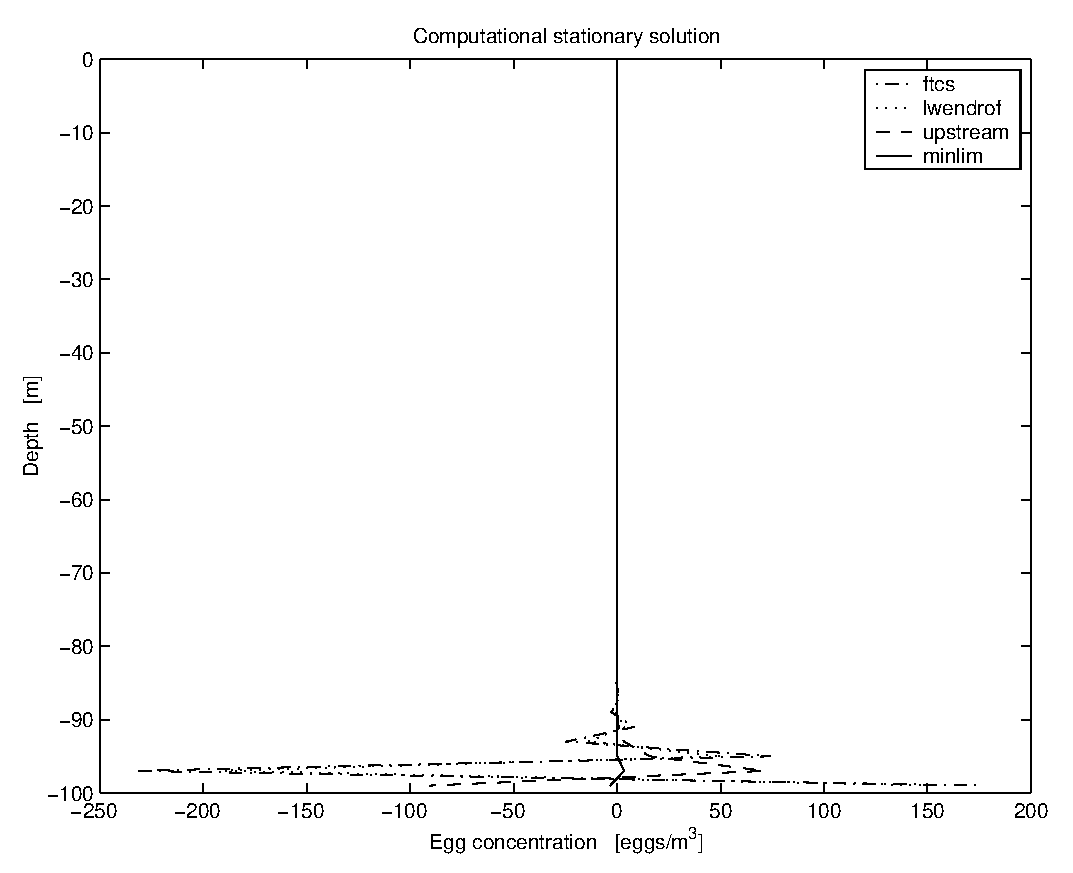
\includegraphics[height=8cm]{ex3b}
\end{center}
\caption{The errors in the numerical stationary
         solutions above}\label{fig:ex3b}
\end{figure}


The other class of tests is meant to be typical of sinking eggs.
Here the eddy diffusivity is 5 per cent of the above,
$K = 0.0005 \sqmps$ and $w = -0.001 \mps$. 
To plot the exact solution
for a subrange of the water column, an index array is used.
\begin{verbatim}
  B = eggsact(M0,K0,W0);
  II = 41:50;  
  plot(B(II),SE(II))
\end{verbatim}
This figure is given as figure~\ref{fig:ex3c}.

The corresponding numerical solutions ($\edb{dz} = 2 \m$, $\edb{dt} =
120 \s$) are shown in figure~\ref{fig:ex3d}. Both the FTCS and the
Lax-Wendroff scheme have produced oscillations and negative values.
The upstream solution is quite smeared out, while the flux limited
method seem to perform quite well. The table for this run is
tab~\ref{tab:ex3sinc}.


\begin{figure}
\begin{center}
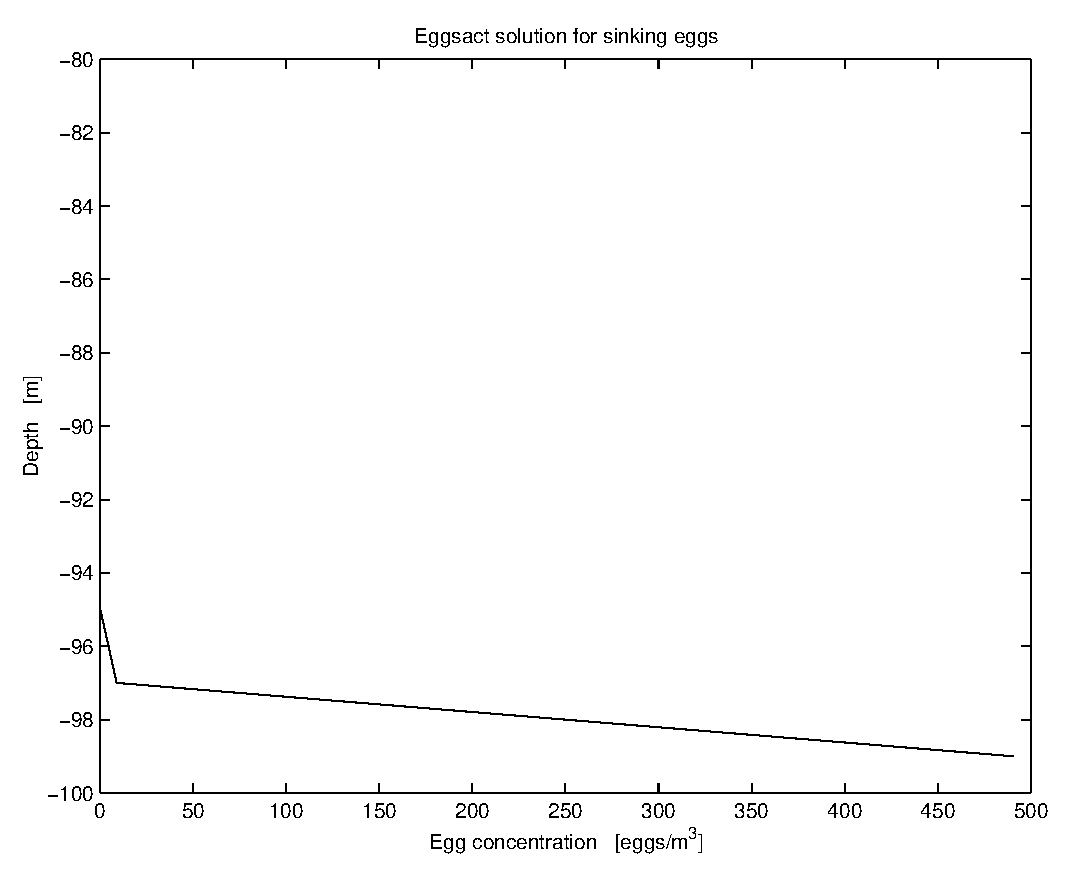
\includegraphics[height=8cm]{ex3c}
\end{center}
\caption{The exact stationary solution with%
     $K = 0.0005 \sqmps$, $w = -0.001 \mps$,%
     $\edb{dz} = 2 \m$}\label{fig:ex3c}
\end{figure}

\begin{table}[h]
\begin{center}
\begin{tabular}{||l|r|r|r|r||}
\hline
    &  RMSE  & E-mean & E-std & CPU-time \\
\hline
ftcs     & 42.549 & -0.537 & -0.640 &  8.6  \\
lwendrof & 35.038 & -0.477 & -0.640 &  8.5  \\
upstream & 16.466 & -0.463 &  0.618 &  8.6  \\
fluxlim  &  0.718 & -0.014 & -0.022 & 32.8  \\
\hline
\end{tabular}
\end{center}
\caption{Results from standard sinking run}\label{tab:ex3sinc}
\end{table}

\begin{figure}
\begin{center}
\includegraphics[height=8cm]{ex3d}
\end{center}
\caption{The numerical stationary solutions with parameters,
     $K = 0.0005 \sqmps$, $w = -0.001 \mps$, $\edb{dz} = 2 \m$, 
     $\edb{dt} = 120 \s$}\label{fig:ex3d}
\end{figure}


\clearpage

\section{Example 4, Terminal egg velocity}

This example verifies and demonstrates the function \edbi{eggvel} for
computing the terminal egg velocities.  The script is \edbi{velex} in
the example directory. Incluided in this example is also the script
\edb{visklsq} which performs the least squares regression used to
derive formula~\eqref{eq:molvisc} for the dynamic molecular viscosity.

First some necessary constant are defined,
\begin{verbatim}
  mu = 1.6e-3;         % Dynamic molecular viscosity 
  g = 9.81;            % Acceleration due to gravity 
  rho = 1027;          % Density of sea water
\end{verbatim}
%% Sjekk korrekt verdi for mu
then the maximum egg diameter \edb{Dmax} for application of
Stokes' formula can be plotted
\begin{verbatim}
  drho = [0.1:0.1:5];      % Range of density differences 
  Dmax = ( 9 * mu^2 ./ (rho * g * drho) ).^(1/3); 
  plot(drho, Dmax * 1000)  % Use mm as unit 
\end{verbatim}

As a verification of the implementation of the formulas in 
\edbi{eggvel}, figure~1 from Sundby \shortcite{sund83} will be
reproduced.
\begin{verbatim}
  d = [0:0.1:5];   % Range of diameters (in mm) 
  hold on 
  axis([0 5 0 5]); 
  for drho = [0.25 0.5 1:6]  % The values of drho used by Sundby 
    W = eggvel(drho * ones(size(d)), d/1000, mu); 
    plot(d, W*1000, 'g')
  end
\end{verbatim}
The expression \edb{drho*ones(size(d))} is required to make \edb{drho}
into an array of the same shape as \edb{d}, as required by
\edb{eggvel}. The factors 1000 converts between \mm\ and \m.
The lines $Re = 0.5$ and $Re = 5.0$ are added in red colour.
This figure is shown as fig.~\ref{fig:ex4a}.
\begin{verbatim}
  d(1) = [];          % Remove d(1) to prevent division by zero
  W = 0.5 * mu ./ (rho * d/1000); 
  W = 1000 * W;       % Convert to mm/s 
  hold on 
  plot(d, W, 'r');    % Re = 0.5 
  plot(d, 10*W, 'r'); % Re = 5.0 
  hold off 
\end{verbatim}


\begin{figure}
\begin{center}
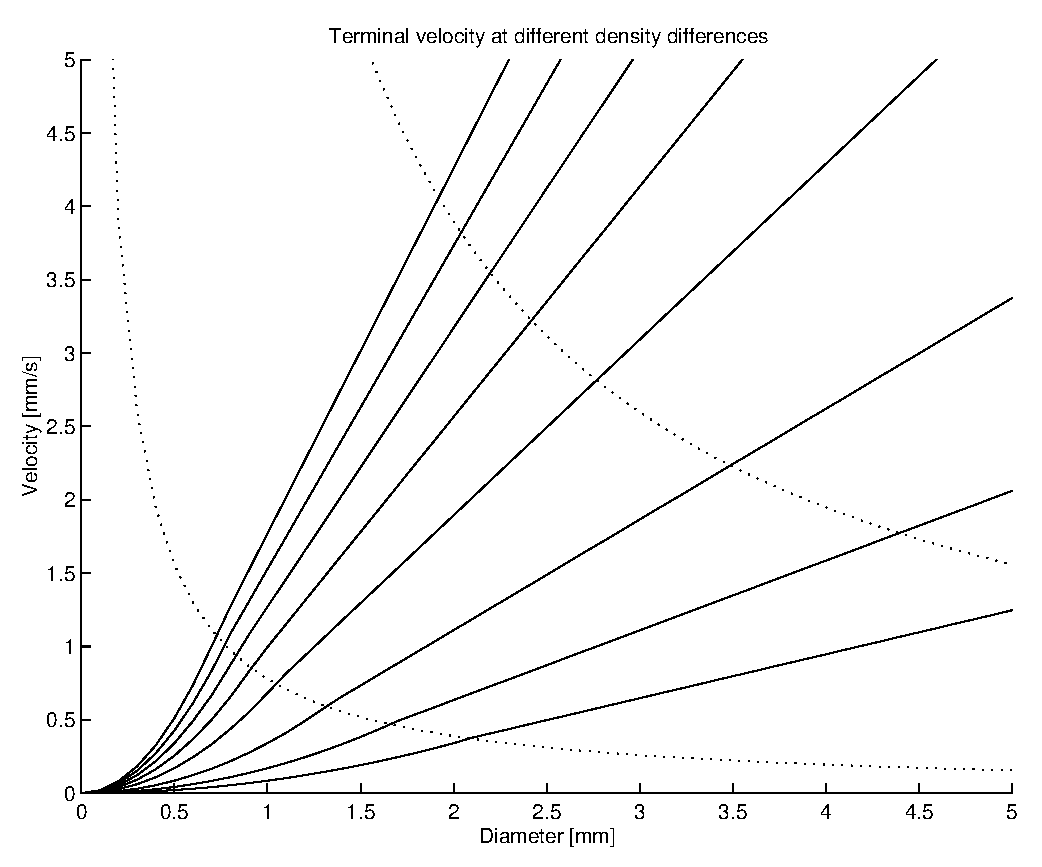
\includegraphics[height=8cm]{ex4a}
\end{center}
\caption{Terminal velocity for different density differences}\label{fig:ex4a}
\end{figure}


Another way of visualizing the \edbi{eggvel} function is to make a
table and make a contour plot of it. The rest of this example is for
MATLAB only.  Tables for \edb{W} and \edb{Re} are made by the
following commands,
\begin{verbatim}
  d = [0:0.1:4];      % mm 
  drho = [0:0.2:6];   % kg/m^3 
  dtab = ones(size(drho))' * d / 1000;  % d constant in colums 
  drhotab = drho' * ones(size(d));  % drho constant in rows  
  [W Re] = eggvel(drhotab, dtab); 
\end{verbatim}
The contour plot is made by.
\begin{verbatim}
  cl = [0.1:0.1:0.5 1.0:0.5:3.0 4.0:9.0]; % Contour levels 
  c = contour(d, drho, 1000*W, cl, 'g'); 
  clabel(c)
\end{verbatim}
Add the same lines $Re = 0.5$ and $Re = 5.0$ in red as above.
\begin{verbatim}
  hold on 
  cl = [0.5 5.0]; 
  contour(d, drho, Re, cl, 'r'); 
  hold off
\end{verbatim}
A 3D view of the velocity surface can also be plotted.
\begin{verbatim}
  surf(d, drho, 1000*W) 
\end{verbatim}

\begin{figure}
\begin{center}
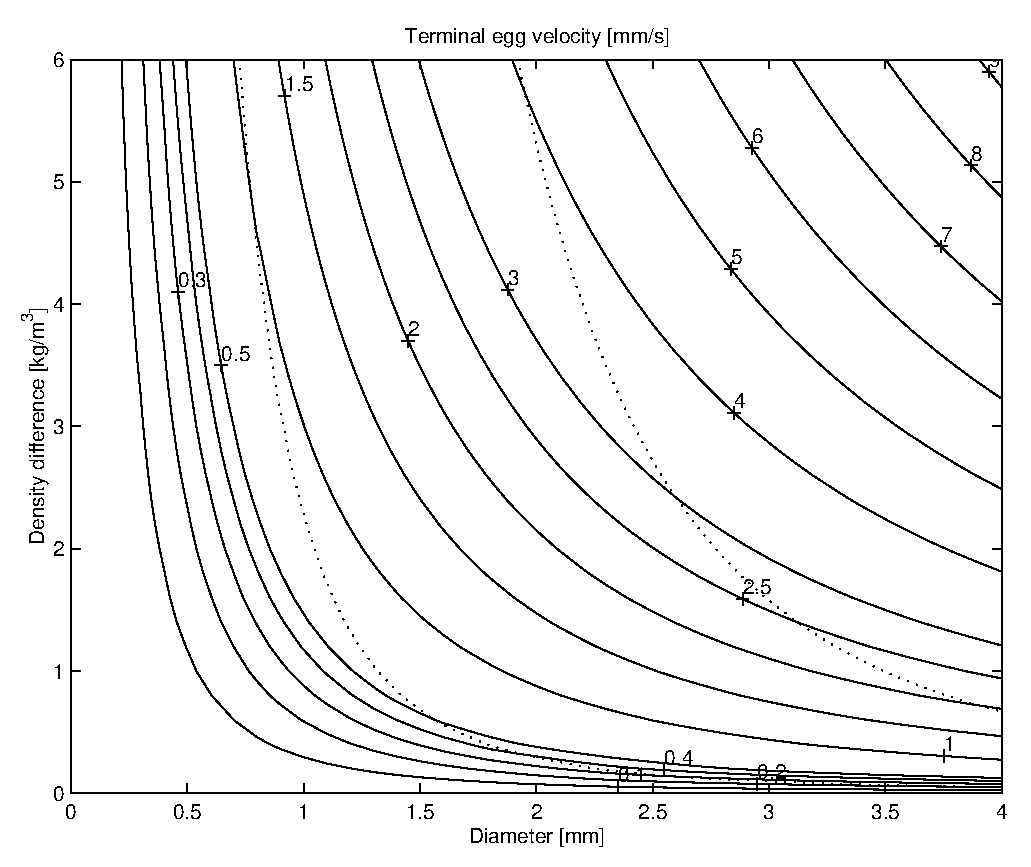
\includegraphics[height=8cm]{ex4b}
\end{center}
\caption{Terminal velocity contours}\label{fig:ex4b}
\end{figure}


Systems like MATLAB and Octave are well suited for fitting functions
to data. The script \edbi{visklsq} demonstrates how to fit a
polynomial, quadratic in $T$ and linear in $S$ to
table~\ref{tab:molvisc} by the method of least squares\index{least
squares}.  Some array manipulation must first be done to obtain
three column vectors \edb{SI}, \edb{TI} and \edb{B} with corresponding
values of salinity, temperature and viscosity. With $\edb{MN} = 35 = 5
\times 7$, the normal matrix is simply
\begin{verbatim}
  A = [ones(MN) TI  TI.^2 SI];  
\end{verbatim}
In MATLAB the vector \edb{X} of coefficients is found by
\begin{verbatim}
  V = eye(MN);       % Covariance matrix = identity 
  X = lscov(A,B,V);  
\end{verbatim}
in Octave the same task is done by
\begin{verbatim}
  X = ols(B,A);
\end{verbatim}


\section{Example 5, Non-constant coefficients}

This example illustrates how to use several egg groups on a transient
problem with non-constant coefficients. It also provides a verification of
parts of the toolbox by reproducing results by Westg{\aa}rd \shortcite{west89}.
The model is contained in the script \edbi{runex5}. The results are
visualized by the scripts \edbi{plotex5} and by animation in
\edbi{animex5}.

The problem is the first example from \cite{west89}. The bottom depth
is 100\m\ and a grid size of 2\m\ is used.
\begin{verbatim}
  ve_init
  ve_grid(100,2)
\end{verbatim}
There is a pycnocline at 50\m, with temperature 7\degC\ and salinity 34
above and temperature 5\degC\ and salinity 35 below.
\begin{verbatim}
  I25 = ones(25,1);        
  S(1:25) = 34*I25; S(26) = 34.5; S(27:51) = 35*I25;
  T(1:25) =  7*I25; T(26) =  6  ; T(27:51) =  5*I25;
\end{verbatim}
The wind speed is 5\mps. The turbulent eddy viscosity in the upper
layer is computed by a formula form Sundby \shortcite{sund83}. The
turbulence in the lower layer is $1/10$ of the value in the upper
layer.
\begin{verbatim}
  Wind = 5;
  K0 = (76.1 + 2.26*Wind^2) * 1e-4;
  K(1:25) = K0*I25; K(26) = 0.55*K0; K(27:51) = 0.1*K0*I25;
\end{verbatim}
There are two groups of eggs, one with a diameter of 1.5\mm\ and
neutral buoyancy corresponding to 33 psu, and the other with a
diameter of 1.3\mm\ and neutral salinity 36 psu. The tool
\edbi{eggvelst} is used to compute the velocity profiles.
\begin{verbatim}
  d1  = 0.0015;
  Se1 = 33;
  W1  = eggvelst(S, T, d1, Se1); 
  d2  = 0.0013;
  Se2 = 36;
  W2  = eggvelst(S, T, d2, Se2); 
\end{verbatim}

The number of eggs are 55 in each group and the initial distribution
is the same step function in each group. The arrays \edb{A1} and
\edb{A2} are used for the concentrations within the groups.
\begin{verbatim}
  I10 = ones(10,1);
  A1( 1:10) = 0*I10;
  A1(11:20) = 0.75*I10;
  A1(21:30) = 1.25*I10;
  A1(31:40) = 0.75*I10;
  A1(41:50) = 0*I10;
  % Use the same initital distribution for group 2
  A2 = A1;
  % Save the intial distributions for later use.
  A10 = A1; A20 = A2;
  A0 = A10 + A20;
\end{verbatim}

The model is here run by the Lax-Wendroff scheme with a time step of 120\s\
and saving the result every 2nd hour. The total simulation time is 96
hours. 
\begin{verbatim}
  for t = 1:nout
    A1 = lwendrof(A1,K,W1,nstep,dt);
    X1(:,t) = A1;
    A2 = lwendrof(A2,K,W2,nstep,dt);
    X2(:,t) = A2;
  end
\end{verbatim}
Finally the results from the two groups are added,
\begin{verbatim}
  X = X1 + X2;
\end{verbatim}

\begin{figure}
\begin{center}
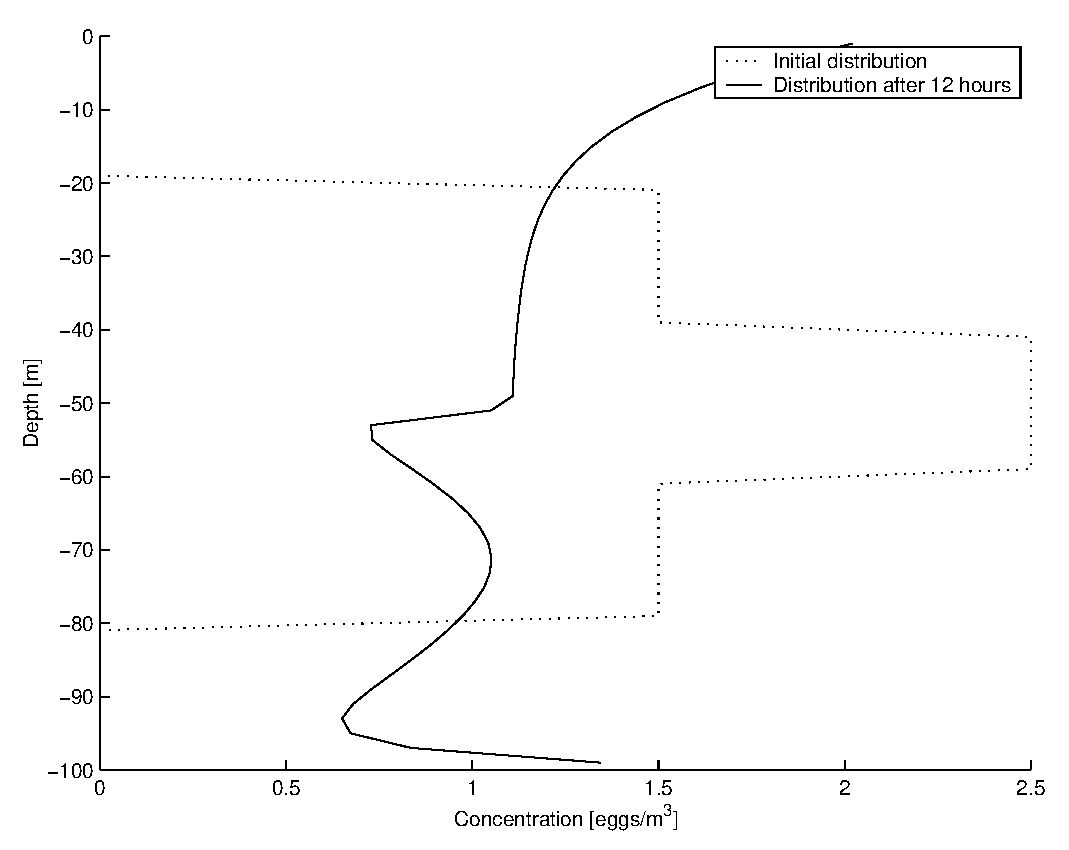
\includegraphics[height=8cm]{ex5a}
\end{center}
\caption{Figure 1 from Westg{\aa}rd (1989)}\label{fig:ex5a}
\end{figure}


Visualising the results with \edb{plotex5} the first task is to
reproduce figure 1 from Westg{\aa}rd \shortcite{west89}.
\begin{verbatim}
  t12 = 12 / outstep;
  hold on;
  plot(A0, ZE, 'y');        % The start distribution   
  plot(X(:,t12), ZE, 'g');  % After 12 hours
\end{verbatim}
This result is depicted in Fig.~\ref{fig:ex5a}.


With non-constant coefficients the function \edbi{sstate} must be used
to calculate the stationary solution.
\begin{verbatim}
  Y1 = sstate(M1,K,W1);
  Y2 = sstate(M2,K,W2);
  Y = Y1 + Y2;
\end{verbatim}
Adding this to the previous figure, gives Fig.~\ref{fig:ex5b}.
\begin{verbatim}
  plot(Y, ZE, 'r'); 
\end{verbatim}

\begin{figure}[h]
\begin{center}
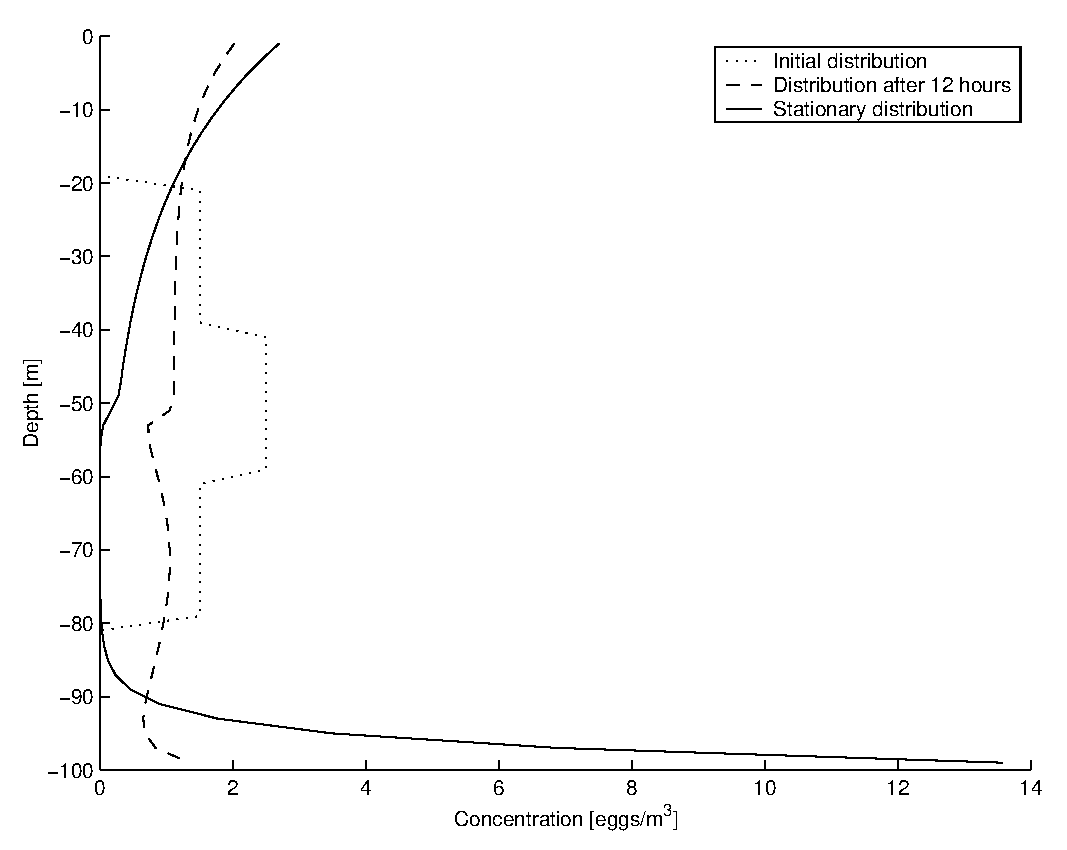
\includegraphics[height=8cm]{ex5b}
\end{center}
\caption{Initial, 12 hour and stationary limit solution}\label{fig:ex5b}
\end{figure}

In addition \edb{plotex5} and \edb{animex5} show more details on the
time evolution. For this example the steady state solution is reached
after approximately 80 hours.



\section{Example 6, Halibut eggs, the transient problem}

 
In this and the next two examples, eggs of Atlantic halibut
\emph{(Hippoglossus hippoglossus)} will be considered
in deeps fjords in northern Norway. Data on egg diameter and egg
salinity are taken from \citep{haug84}.  Synthetic vertical profiles,
representative for the area, of temperature, salinity and vertical
mixing have been constructed by S.~Sundby (pers.~comm.).

This example goes further towards developing a model application from
VertEgg. The main script \edbi{runex6} is initiated from the set-up file
\edb{runex6.sup}. The physical setting and initial egg distribution are
also read from files.
The model script is meant to be a prototype simulation model.
It should be easy to modify for similar simulations.
The script \edbi{plotini} is
used to plot the  physical and numerical situation before the
simulation, while \edbi{plotgrp3} and \edbi{plotres} are used for 
postprocessing of the model results. 

First the physical profiles will be plotted. 
The profiles are read from file and thereafter interpolated to
the flux points. The variable names are \edb{S} for salinty,
\edb{T} for temperature and \edb{K} for vertical mixing coefficient.
Several profiles are
combined into one figure by the Matlab command \edbi{subplot}.
\begin{verbatim}
  subplot(1,3,1)
  plot(S,ZF)
  title('Salinity')
  subplot(1,3,2)
  plot(T,ZF)
  title('Temperature')
  subplot(1,3,3)
  semilogx(K,ZF)   % Logarithmic X-axis
  title('Vertical mixing')
\end{verbatim}
The result is shown in fig.~\ref{fig:ex6a}

\begin{figure}[!htb]
\begin{center}
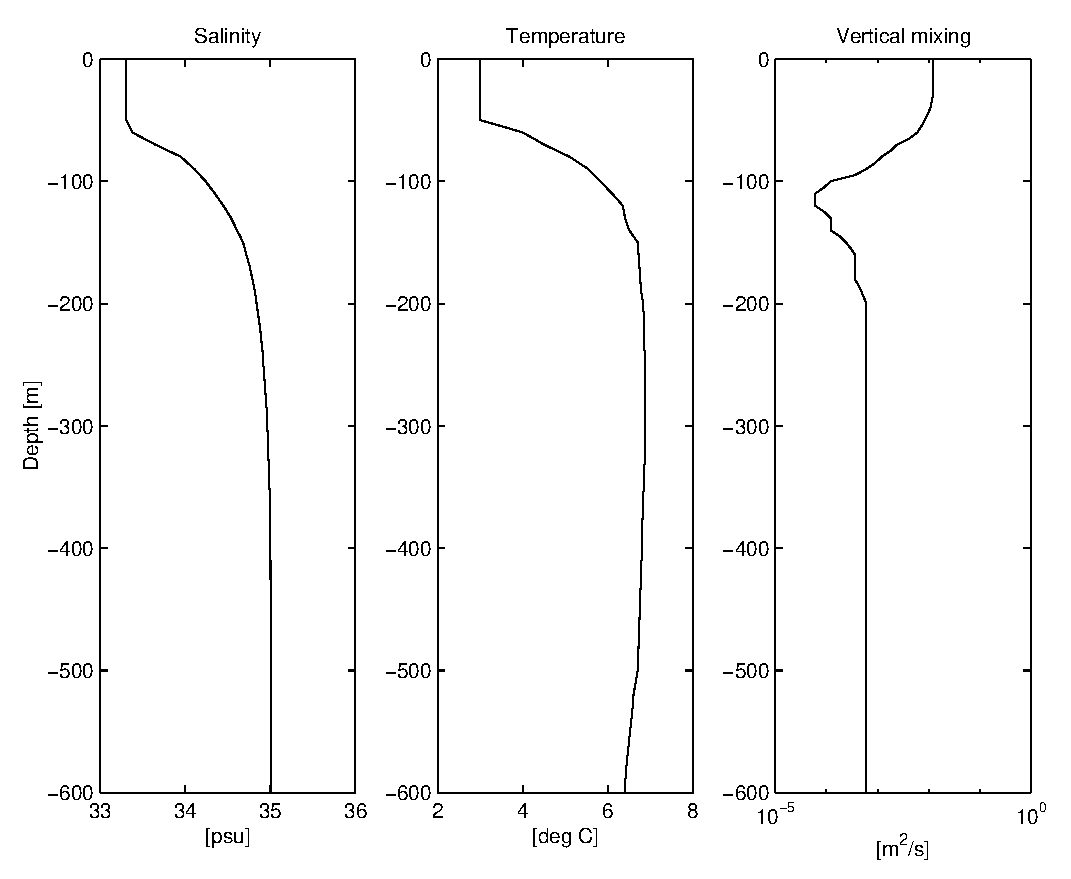
\includegraphics[height=8cm]{ex6a}
\end{center}
\caption{Vertical profiles of salinty, temperature and 
         vertical eddy viscosity}
\label{fig:ex6a}
\end{figure}

With the values 34.5 psu for egg salinity and egg diameter 3.2\mm,
\edbi{eggvelst} can be used to compute the egg velocity. Thereafter
the stationary solution with integrated density 100 eggs/m$^3$ can be
computed by \edbi{sstate}.
\begin{verbatim}
  eggsal = 34.5;
  eggdiam = 3.2;
  W = eggvelst(S,T,eggdiam/1000.0,eggsal);
  M = 100;
  ASS = sstate(M,K,W);
\end{verbatim}
The profiles are plotted in figure~\ref{fig:ex6b}. The vertical dotted
line in the left indicate zero velocity. 

\begin{figure}[!htb]
\begin{center}
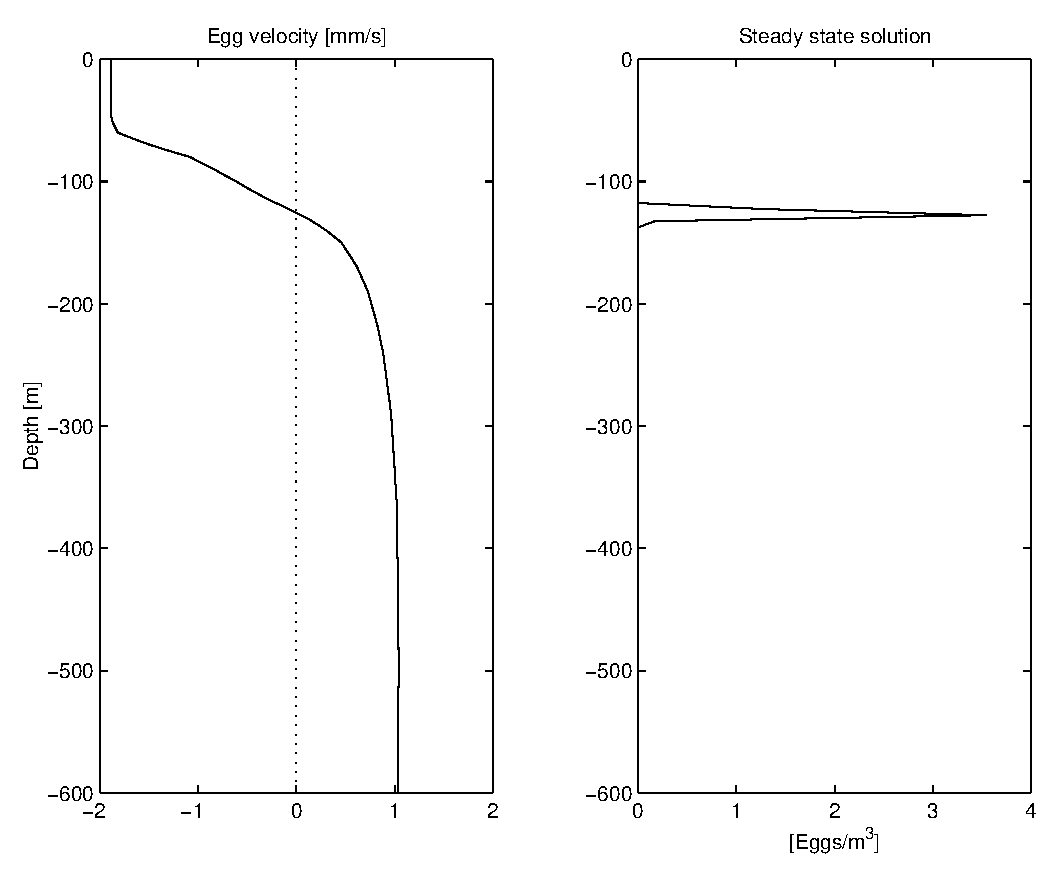
\includegraphics[height=8cm]{ex6b}
\end{center}
\caption{Egg velocity and stationary ditribution}
\label{fig:ex6b}
\end{figure}

The neutral salinity 34.5 occur at approximately 125\m\ depth, in the
pycnocline layer where the vertikal mixing coefficient is very
low. The stationary solution is therefore a very narrow peak at this
depth level.

Before running the transient simulation it is useful to look at the
numerical characteristics of the problem.  With $\Delta z = 5\m$ and
$\Delta t = 600\s$ the profiles are plotted in
figure~\ref{fig:ex6c}. 
All the three linear methods are stable.
However, the methods are not suitable because the high Peclet
numbers give high numerical diffusion in the upstream method and
produce negative values with FTCS and Lax-Wendroff. Therefore the more
time-consuming method \edbi{posmet} is used for the transient
simulations.


\begin{figure}[!htb]
\begin{center}
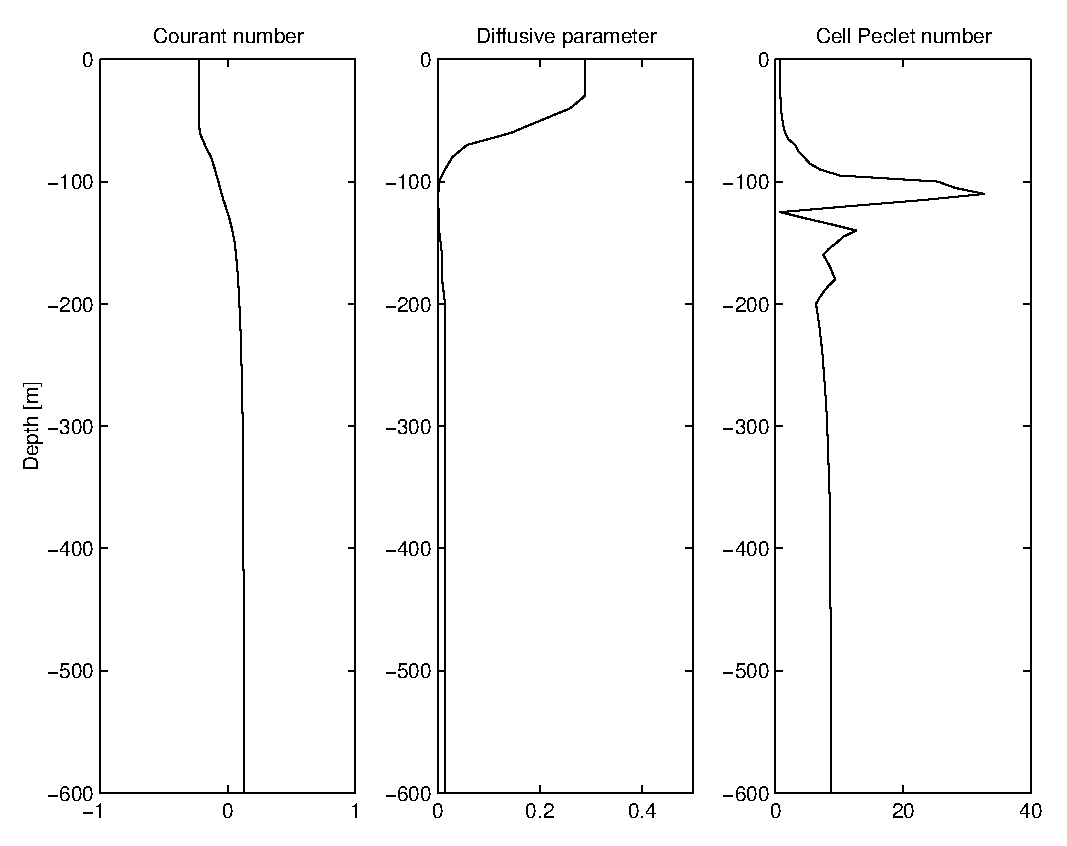
\includegraphics[height=8cm]{ex6c}
\end{center}
\caption{Vertical profiles of Courant number, diffusive parameter 
         and cell Peclet number}
\label{fig:ex6c}
\end{figure}

The model script start by reading the setup-file. Thereafter the
vertical physical profiles are read in and interpolated as above.
Similarly the inital egg distribution is read from file
\edb{halibut.dat} and interpolated to the egg points. 

Initially the eggs are distributed between 500 and 600\m\ depth.
The model is run with space step $\Delta z = 5\m$ and time
step $\Delta t = 10\, \text{minutes}$ as above. 5 egg groups are used,
all with diameter 3.2\mm\ but the neutral salinity vary from 34.3 to
34.7 psu in steps of 0.1. The simulation time is 10 days, and the
results are written to file every 12 hours.

The first post-processing script \edb{plotgrp3} concentrates on egg
group 3, which is neutral at salinity 34.5 psu.  The model output file
\edb{result.dat} is read and the egg profile data every 24 hour
starting with the initial distribution is 
stored in the array \edb{X3}. The command
\begin{verbatim}
  plot(X3,ZE)
\end{verbatim}
plots these daily distributions in fig.~\ref{fig:ex6d}. The numerics
seems to be working, the distributions do not contain negative values
and the eggs are moving upwards a little less then 100\m\ per day
without too much smoothing of the distribution. After 5--6 days the
distribution has reached it equilibrium level and start to concentrate
at this level. After the 10 days, the transient solution is very
similar to the stationary solutions. These solutions are compared in
figure~\ref{fig:ex6e}. The transient solution have a slightly higher
peak consentration.

\begin{figure}[!htb]
\begin{center}
\includegraphics[height=8cm]{ex6d}
\end{center}
\caption{Daily egg distributions from egg group 3}
\label{fig:ex6d}
\end{figure}

\begin{figure}[!htb]
\begin{center}
\includegraphics[height=8cm]{ex6e}
\end{center}
\caption{The distribution after 10 days compared to the
         steady state distribution from \edb{sstate}}
\label{fig:ex6e}
\end{figure}


The script \edbi{plotres} is used for postprocessing the results for
all 5 egg groups. In this case the columns in \edb{X} hold the sum of the
5 concentrations every 12 hour.
Figure~\ref{fig:ex6f} show the distributions for the 5 egg groups
after the 10 days of simulation. 
The solution is a narrow peak for each egg group at their equilibrium
salinity.


\begin{figure}[!htb]
\begin{center}
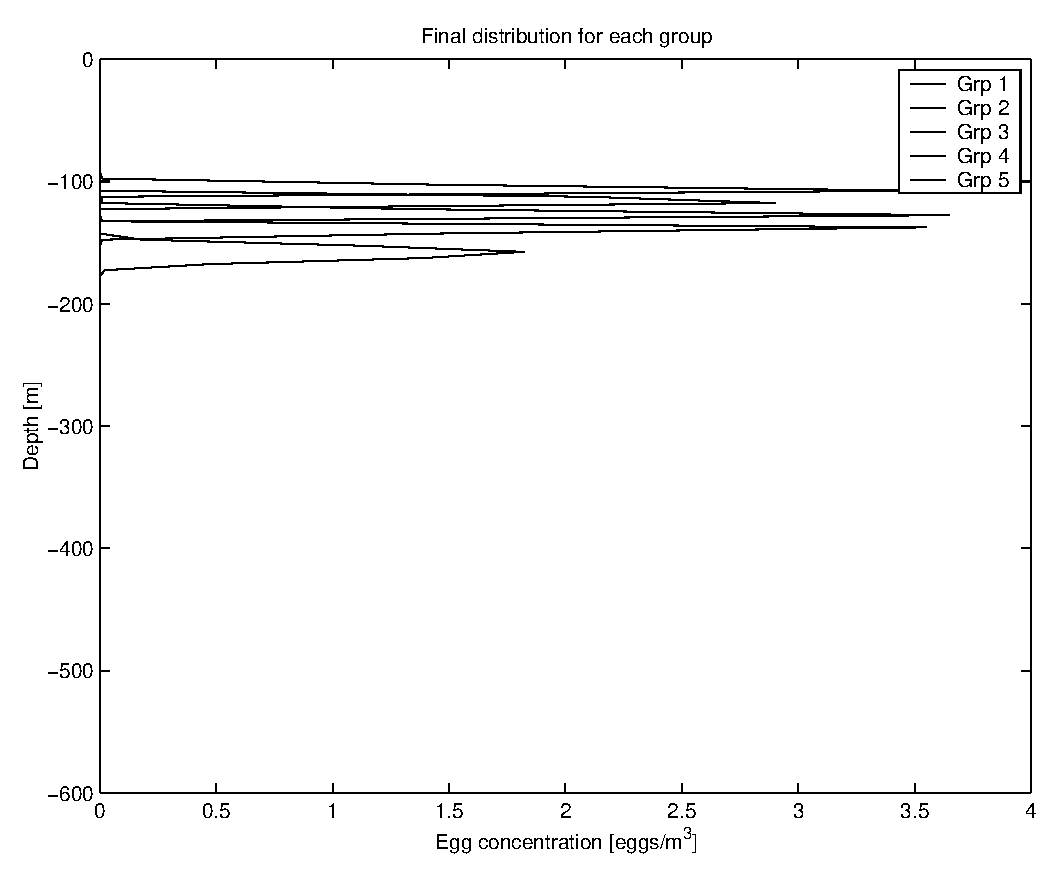
\includegraphics[height=8cm]{ex6f}
\end{center}
\caption{Final distribution of the 5 egg groups}
\label{fig:ex6f}
\end{figure}

The next figure~\ref{fig:ex6g} show the time evolution of the mean
depth of the distributions. Note that although the distance is shorter
the heaviest eggs use longer time to raise to their equilibrium
depth. This confirms unpublished calculations by S.~Sundby.

\begin{figure}[!htb]
\begin{center}
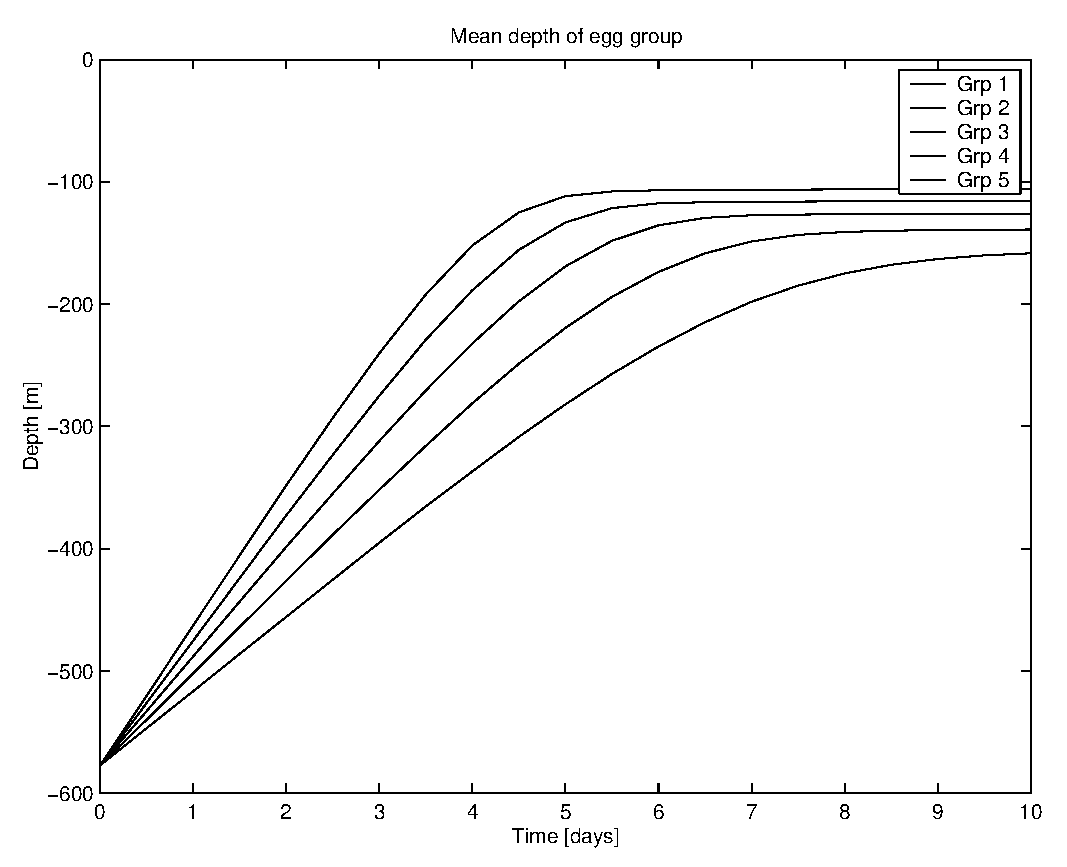
\includegraphics[height=8cm]{ex6g}
\end{center}
\caption{Time evolution of mean depth}
\label{fig:ex6g}
\end{figure}



\section{Example 7, Halibut eggs, Monte Carlo simulation}
\index{Monte Carlo}
{\bfseries Under construction}

In nature, egg diameters and densities are not constant or confined to
a handful of discrete groups. To explore this further it is assumed
that these properties have known statistical distributions.  The paper
\citep{haug84} does not identify the distributions but give ranges for
the values.  For the egg diameter a normal distribution with mean
3.2\mm\ and standard deviation 0.2\mm is used below. For the neutral
salinity of the egg a normal distribution with mean 34.5 psu and
standard deviation 0.2 psu is used. For simplicity it is assumed here
that egg diameter and egg salinity are independent.

In the script \edbi{runex7} a total of \edb{Nprof} egg diameters and 
corresponding egg salinities are
drawn randomly from the distributions above. Thereafter
\edbi{eggvelst} is used to compute the velocity profiles and
\edbi{sstate} computes the vertical distribution. The variable
\edb{Anorm} contains the average of the distributions so far,
normalised so that the vertical integral equal \edb{M} eggs/m$^2$.

The script \edbi{plotex7} is used to plot the results.
With \edb{Nprof} = 1000 the averaged vertical profile is given
in figure~\ref{fig:ex7a}. Nearly all the eggs are found 
between 50 and 300\m\ depth with high concentrations between 
100 and 200\m. Also note the few heavy eggs are  near bottom.

\begin{figure}[!htb]
\begin{center}
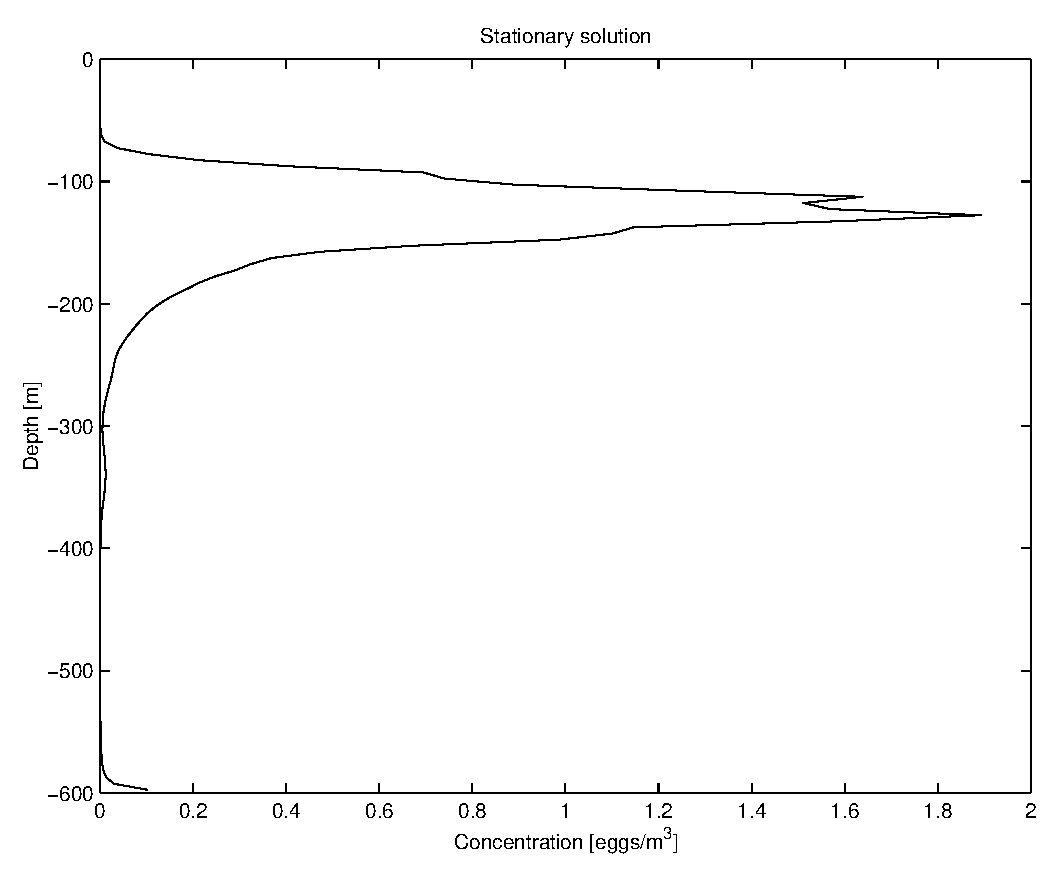
\includegraphics[height=8cm]{ex7a}
\end{center}
\caption{Vertical distribution of eggs from Monte Carlo run}
\label{fig:ex7a}
\end{figure}

Thereafter some statistics of this solution
is computed. Because of the randomness in the Monte Carlo process
these numbers (and the shape of fig.~\ref{fig:ex7a}) may vary from run
to run. In our case we obtain the following numbers. The egg diameters vary
from 2.57 to 3.85\mm\ with mean 3.19\mm\ and standard deviation
0.21\mm. The egg salinities vary from 33.87 to 35.22  with mean
34.50 and standard deviation 0.20 psu. The mean depth of the
distribution is 135.1\m and the standard deviation is 50.7\m.

To visualize the convergence of the Monte Carlo run, the root mean
square deviation of the normalised distribution after $i-1$ and $i$
iterations are saved in the array $R(i)$. Figure~\ref{fig:ex7b}
show the evolution of $R$ on a logarithmic scale. The convergence is 
quite slow, and 1000 samples may be too few. This explains why the
shape of the distribution may vary from run to run.

\begin{figure}[!htb]
\begin{center}

\includegraphics[height=8cm]{ex7b}
\end{center}
\caption{Development of the root mean square increment}
\label{fig:ex7b}
\end{figure}

\section{Example 8, Halibut eggs with spawning and hatching terms}
{\bfseries Under construction}





\chapter{Reference Manual --- VertEgg Version 0.9}

\section{Overview of the Toolbox}

The VertEgg toolbox  presently contain  the following tools,
grouped here according to functionality.

\begin{itemize}
  \item Initialise VertEgg
    \begin{itemize}
      \item \edb{ve\_init}
      \item \edb{ve\_grid(Hcol, dz)}
    \end{itemize}  
  \item Make initial egg distribution
    \begin{itemize}
      \item \edb{spawn(M, Z)}
      \item \edb{ve\_rand(M)}
    \end{itemize}  
  \item Compute the stationary solution
    \begin{itemize}
      \item \edb{eggsact(M, K, W, Z)}
      \item \edb{srcsact(K, W, P, alpha)}
      \item \edb{sstate(M, K, W)}
    \end{itemize}  
  \item Solve the transient problem numerically
    \begin{itemize}
      \item \edb{fluxlim(A0, K, W, nstep, dt, P, alpha)}
      \item \edb{ftcs(A0, K, W, nstep, dt, P, alpha)}
      \item \edb{lwendrof(A0, K, W, nstep, dt, P, alpha)}
      \item \edb{upstream(A0, K, W, nstep, dt, P, alpha)}
    \end{itemize} 
  \item Compute terminal egg velocity
    \begin{itemize}
      \item \edb{dens0(S, T)}
      \item \edb{eggvel(drho, d, mu)}
      \item \edb{eggvelst(S, T, d, Se)}
      \item \edb{molvisc(S, T)}
    \end{itemize} 
  \item Analyse distributions
    \begin{itemize}
      \item \edb{eggmom(A, p)}
      \item \edb{ve\_drint(A, z1, z2)}
      \item \edb{ve\_int(A)}
      \item \edb{ve\_mean(A)}
      \item \edb{ve\_std(A)}
      \item \edb{ve\_rmsd(A, B)}
    \end{itemize} 
\end{itemize}


\section{Description of the Tools}


{\parindent=0pt


\thead{dens0}{Sigma-T of sea water at zero pressure}

\begin{tdesc}
\item[Usage] \edb{sigma = dens0(S, T)}
\item[Input]
  \begin{vartab}
    \edb{S}  \> : \> Salinity     \>   [psu]   \\
    \edb{T}  \> : \> Temperature  \>   [\degC] 
  \end{vartab}
  \edb{S} and \edb{T} may be arrays of the same shape.
\item[Output]
  \begin{vartab}
    \edb{sigma} \> : \> Sigma-T value \>  [\kgpcum] 
  \end{vartab}
  \edb{sigma} is an array of the same shape as \edb{S} and \edb{T}.
\item[Description] \mbox{}\\
  \edb{dens0} computes the $\sigma_T$ value (density - 1000)
  of sea water at zero pressure.
  The density is computed by the international equation
  of state for sea water, UNESCO, 1980.
\end{tdesc}


\thead{eggmom}{Moment of egg distribution}

\begin{tdesc}
\item[Usage] \edb{M = eggmom(A, p)}
\item[Input]
  \begin{vartab}
  \edb{A}   \> : \> Egg distribution \>  [eggs/m$^3$] \\
  \edb{p}   \> : \> Order of moment  
  \end{vartab}
  \edb{A} must be a matrix where the columns live on egg-points,
  but a row-vector at egg-points is also accepted,
  \edb{size(A) = (Ncell x n)} or \edb{(1 x Ncell)}
\item[Output]
  \begin{vartab}
  \edb{M}  \>  : \> The \edb{p}-th moment of \edb{A} \> [eggs m$^{p-2}$]
  \end{vartab}
  If \edb{A} is a matrix of size \edb{(Ncell x n)}, \edb{M} becomes a 
  row-vector of length n containing the moments of
  the columns of \edb{A}. \edb{p} must not be negative.
\item[Description]\mbox{}\\
  Computes the \edb{p}-th moment of the egg-distribution \edb{A},
  \begin{displaymath}
      M = \int^0_{-H} z^p a(z) dz
  \end{displaymath}
   where $a(z)$ is the piecewise constant function 
   $a(z) = \edb{A(i)}$ for $\edb{ZF(i+1)} < z < \edb{ZF(i)}$.
   If \edb{A} is a matrix, the moments of the columns are
   calculated.
\end{tdesc}


\thead{eggsact}{Exact stationary solution, const. coeff.}

\begin{tdesc}
\item[Usage] \edb{A = eggsact(M, K, W, Z)}
\item[Input]
  \begin{vartab}
  \edb{M}   \> : \> Vertical integrated concentration \>  [eggs/m$^2$] \\
  \edb{K}   \> : \> Eddy diffusivity     \> [\sqmps] \\
  \edb{W}   \> : \> Terminal velocity   \>  [\mps] \\
  \edb{Z} (opt) \> : \> Vertical coordinate  \> [\m] 
  \end{vartab}
  \edb{M}, \edb{K}, \edb{W} are scalars. \edb{Z} can be arbitrary array.
  IF \edb{Z} is omitted, \edb{ZE} is used as vertical coordinates.
\item[Output]
  \begin{vartab}
  \edb{A}     \>  : \> Concentration at depth \edb{Z} \> [eggs/m$^3$]
  \end{vartab}
  If \edb{Z} is present, \edb{size(A) = size(Z)},
  otherwise, \edb{size(A) = size(ZE)}.
\item[Description]
   Computes the exact stationary solution of the
   convection diffusion equation with constant
   eddy diffusivity \edb{K} and velocity \edb{W}.
   If \edb{Z} is present, returns array of pointwise values.
   If \edb{Z} is not present, returns exact cell averages.
\end{tdesc}

\thead{eggvel}{Terminal egg velocity}

\begin{tdesc}
\item[Usage] \edb{[W, Re] = eggvel(drho, d, mu)}
\item[Input]
   \begin{vartab}
   \edb{drho}  \> : \> Buoyancy of egg  \> [\kgpcum] \\
   \edb{d}     \> : \> Diameter of egg  \> [\m] \\
   \edb{mu} (opt) \> : 
         \> Dynamic molecular viscosity \>   [kgm$^{-1}$s$^{-1}$] 
   \end{vartab}
   \edb{drho}, \edb{d} and \edb{mu} can be matrices (of the same shape).
   \edb{mu} can be also be a scalar or omitted.
   The sign of \edb{drho} is positive if the egg is ascending,
   \edb{drho} = Density of water - density of egg. With only two arguments,
   a default value 0.0016 is used for \edb{mu}. 
\item[Output]
  \begin{vartab}
  \edb{W}   \> : \> Terminal velocity  \> [\mps] \\
  \edb{Re} (opt) \> : \> Reynolds number
  \end{vartab}
\item[Description]
  Computes the terminal velocity of a small sphere in sea water
  by the formulas in Stokes' or Dallavalles formula.
\end{tdesc}


\thead{eggvelst}{Egg velocity from salinity and temperature}

\begin{tdesc}
\item[Usage] \edb{[W, Re] = eggvelst(S, T, d, Se)}
\item[Input]
  \begin{vartab}
  \edb{S}  \>  : \> Salinity of the environment \> [psu]   \\
  \edb{T}  \>  : \> Temperature                 \> [\degC] \\
  \edb{d}  \>  : \> Egg diameter                \> [m]     \\
  \edb{Se} \>  : \> Egg salinity                \> [psu]
  \end{vartab}
  All arguments can be arrays of the same shape.
  Alternatively \edb{d} and/or \edb{Se} may be scalars.
\item[Output]
  \begin{vartab}
  \edb{W}    \> : \> Terminal velocity  \> [\mps] \\
  \edb{Re} (opt) \> : \> Reynolds number
  \end{vartab}
\item[Description]\mbox{}\\
  Computes the terminal egg velocity given the hydrography
  of the environment and the salinity \edb{Se} where the egg is
  neutral buoyant.
\end{tdesc}

\thead{fluxlim}{Numerical integration of transport equation}

\begin{tdesc}
\item[Usage] \edb{A = fluxlim(A0, K, W, nstep, dt, P, alpha)}
\item[Input]
  \begin{vartab}
  \edb{A0}  \> : \> Start concentration \>  [eggs/m$^3$] \\
  \edb{K}   \> : \> Eddy diffusivity    \>  [\sqmps]  \\
  \edb{W}   \> : \> Terminal velocity   \>  [\mps]  \\
  \edb{nstep}  \> : \> Number of integration steps \\
  \edb{dt}     \> : \> Time step           \>  [s] \\
  \edb{P}     (opt) \> : \> Spawning term       \>  [eggs/m$^3$/s] \\
  \edb{alpha} (opt) \> : \> Loss coefficient \> [1/s] 
  \end{vartab}
  \edb{A0} lives at the egg-points, \edb{size(A0) = (Ncell x 1)}.
  \edb{K} and \edb{W} live at the flux-points, \edb{size = (Ncell+1 x1)}.
  If \edb{P} and \edb{alpha} are present, they also live at the egg-points.
  If \edb{P} and \edb{alpha} are missing, the source term is ignored. 
\item[Output]
  \begin{vartab}
  \edb{A} \>  : \> Result concentration \> [eggs/m$^3$]
  \end{vartab}
  \edb{A} lives at egg-points in the same way as \edb{A0}
\item[Description]\mbox{}\\
  Integrates the convection-diffusion equation by the 
  flux-limited method. Starting with the concentration 
  in \edb{A0} nstep integration steps  are performed. 
  The result is saved in \edb{A}.
\end{tdesc}


\thead{ftcs}{Numerical integration of transport equation}

\begin{tdesc}
\item[Usage] \edb{A = ftcs(A0, K, W, nstep, dt, P, alpha)}
\item[Input]
  \begin{vartab}
  \edb{A0}  \> : \> Start concentration \>  [eggs/m$^3$] \\
  \edb{K}   \> : \> Eddy diffusivity    \>  [\sqmps]  \\
  \edb{W}   \> : \> Terminal velocity   \>  [\mps]  \\
  \edb{nstep}  \> : \> Number of integration steps \\
  \edb{dt}     \> : \> Time step           \>  [s] \\
  \edb{P}     (opt) \> : \> Spawning term       \>  [eggs/m$^3$/s] \\
  \edb{alpha} (opt) \> : \> Loss coefficient \> [1/s] 
  \end{vartab}
  \edb{A0} lives at the egg-points, \edb{size(A0) = (Ncell x 1)}.
  \edb{K} and \edb{W} live at the flux-points, \edb{size = (Ncell+1 x1)}.
  If \edb{P} and \edb{alpha} are present, they also live at the egg-points.
  If \edb{P} and \edb{alpha} are missing, the source term is ignored. 
\item[Output]
  \begin{vartab}
  \edb{A} \>  : \> Result concentration \> [eggs/m$^3$]
  \end{vartab}
  \edb{A} lives at egg-points in the same way as \edb{A0}
\item[Description]\mbox{}\\
  Integrates the convection-diffusion equation by the 
  forward time central space (FTCS)  method. Starting 
  with the concentration in \edb{A0} nstep integration steps 
  are performed. The result is saved in \edb{A}.
\end{tdesc}




\thead{lwendrof}{Numerical integration of transport equation}

\begin{tdesc}
\item[Usage] \edb{A = lwendrof(A0, K, W, nstep, dt, P, alpha)}
\item[Input]
  \begin{vartab}
  \edb{A0}  \> : \> Start concentration \>  [eggs/m$^3$] \\
  \edb{K}   \> : \> Eddy diffusivity    \>  [\sqmps]  \\
  \edb{W}   \> : \> Terminal velocity   \>  [\mps]  \\
  \edb{nstep}  \> : \> Number of integration steps \\
  \edb{dt}     \> : \> Time step           \>  [s] \\
  \edb{P}     (opt) \> : \> Spawning term       \>  [eggs/m$^3$/s] \\
  \edb{alpha} (opt) \> : \> Loss coefficient \> [1/s] 
  \end{vartab}
  \edb{A0} lives at the egg-points, \edb{size(A0) = (Ncell x 1)}.
  \edb{K} and \edb{W} live at the flux-points, \edb{size = (Ncell+1 x1)}.
  If \edb{P} and \edb{alpha} are present, they also live at the egg-points.
  If \edb{P} and \edb{alpha} are missing, the source term is ignored. 
\item[Output]
  \begin{vartab}
  \edb{A} \>  : \> Result concentration \> [eggs/m$^3$]
  \end{vartab}
  \edb{A} lives at egg-points in the same way as \edb{A0}
\item[Description]\mbox{}\\
  Integrates the convection-diffusion equation by the 
  Lax-Wendroff method. Starting with the concentration
  in \edb{A0} nstep integration steps are performed. The 
  result is saved in \edb{A}.
\end{tdesc}

\thead{molvisc}{Dynamical molecular viscosity of sea water}

\begin{tdesc}
\item[Usage] \edb{mu = molvisc(S, T)}
\item[Input]
  \begin{vartab}
    \edb{S}     \> : \> Salinity     \>   [psu]   \\
    \edb{T}     \> : \> Temperature  \>   [\degC] 
  \end{vartab}
  \edb{S} and \edb{T} may be arrays of the same shape.
\item[Output]
  \begin{vartab}
    \edb{mu} \> : \> Dynamic molecular viscosity \>  [kgm$^{-1}$s$^{-1}$] 
  \end{vartab}
  \edb{mu} is an array of the same shape as \edb{S} and \edb{T}.
\item[Description] \mbox{}\\
  Computes the dynamic molecular viscosity by formula~\eqref{eq:molvisc}.
\end{tdesc}


\thead{spawn}{Make concentrated egg distribution}

\begin{tdesc}
\item[Usage] \edb{A = spawn(M, Z)}
\item[Input]
  \begin{vartab}
  \edb{M} \> : \> Vertical integrated concentration \>  [eggs/m$^2$] \\
  \edb{Z} \> : \> Spawning depth              \>       [m]
  \end{vartab}
  \edb{M} and \edb{Z} are scalars.
\item[Output]
  \begin{vartab}
  \edb{A}  \> : \> Egg distribution     \>        [eggs/m$^3$]
  \end{vartab}
  \edb{A} is a column vector, living at the egg points.
\item[Description]\mbox{}\\
  Returns a vertical egg distribution \edb{A} with vertical
  integral \edb{M}, concentrated as much as possible around 
  depth = \edb{Z}.
  If $\edb{ZE(Ncell)} < \edb{Z} < \edb{ZE(1)}$, then \edb{Z = ve\_mean(A)}.
\end{tdesc}


\thead{srcsact}{Stationary solution, const. coeff., source term}

\begin{tdesc}
\item[Usage] \edb{A = srcsact(K, W, P, alpha, Z)}
\item[Input]
  \begin{vartab}
    \edb{K} \> : \> Eddy diffusivity  \>  [\sqmps] \\
    \edb{W} \> : \> Terminal velocity \>  [\mps] \\
    \edb{P} \> : \> Egg production    \>  [eggs/m$^3$/s] \\
    \edb{alpha} \> : \> Egg loss rate  \>       [1/s] \\
    \edb{Z} (opt) \> : \> Vertical coordinate \>  [m]
  \end{vartab}
  \edb{K}, \edb{W}, \edb{P} and \edb{alpha} are scalars. \edb{Z} can 
  be an arbitrary array.
  If \edb{Z} is ommitted, \edb{ZE} is used as vertical coordinate.
\item[Output]
  \begin{vartab}
    \edb{A} \> : \>  Concentration at depth \edb{Z}.  \>   [eggs/m$^3$]
  \end{vartab}
  If \edb{Z} is present, \edb{size(Y) = size(Z)},
  otherwise, \edb{size(Y) = size(ZE)}.
\item[Description]\mbox{}\\
   Computes the exact stationary solution of the
   convection diffusion equation with constant
   eddy diffusivity \edb{K}, velocity \edb{W}, egg production \edb{P}
   and loss rate \edb{alpha}.
   If \edb{Z} is present, returns array of pointwise values.
   If \edb{Z} is not present, returns exact cell averages.
\end{tdesc}


\thead{sstate}{Steady state solution}

\begin{tdesc}
\item[Usage] \edb{A = sstate(M, K, W)}
\item[Input]
  \begin{vartab}
  \edb{M} \>  : \> Vertical integrated concentration \> [eggs/m$^2$] \\
  \edb{K} \>  : \> Eddy diffusivity \> [\sqmps] \\
  \edb{W} \>  : \> Egg velocity   \>  [\mps]
  \end{vartab}
  \edb{M} is scalar, \edb{K} and \edb{W} are column vectors of
  length \edb{Ncell+1}, \edb{K} and \edb{W} live at the flux-points.
\item[Output]
  \begin{vartab}
  \edb{A}    \>  : \> Stationary solution \> [eggs/m$^3$]
  \end{vartab}
  \edb{A} lives at the egg points, \edb{size = (Ncell x 1)}.
\item[Description]\mbox{}\\
  Computes the steady state solution of the convection-
  diffusion equation without source term, with eddy diffusivity 
  \edb{K} and egg
  velocity \edb{W} variable in the water column. 
  The solution is computed by viewing \edb{K} and \edb{W}
  as piecewise constant on the grid cells.
\end{tdesc}


\thead{upstream}{Numerical integration of transport equation}

\begin{tdesc}
\item[Usage] \edb{A = upstream(A0, K, W, nstep, dt, P, alpha)}
\item[Input]
  \begin{vartab}
  \edb{A0}  \> : \> Start concentration \>  [eggs/m$^3$] \\
  \edb{K}   \> : \> Eddy diffusivity    \>  [\sqmps]  \\
  \edb{W}   \> : \> Terminal velocity   \>  [\mps]  \\
  \edb{nstep}  \> : \> Number of integration steps \\
  \edb{dt}     \> : \> Time step           \>  [s] \\
  \edb{P}     (opt) \> : \> Spawning term       \>  [eggs/m$^3$/s] \\
  \edb{alpha} (opt) \> : \> Loss coefficient \> [1/s] 
  \end{vartab}
  \edb{A0} lives at the egg-points, \edb{size(A0) = (Ncell x 1)}.
  \edb{K} and \edb{W} live at the flux-points, \edb{size = (Ncell+1 x1)}.
  If \edb{P} and \edb{alpha} are present, they also live at the egg-points.
  If \edb{P} and \edb{alpha} are missing, the source term is ignored. 
\item[Output]
  \begin{vartab}
  \edb{A} \>  : \> Result concentration \> [eggs/m$^3$]
  \end{vartab}
  \edb{A} lives at egg-points in the same way as \edb{A0}
\item[Description]\mbox{}\\
  Integrates the convection-diffusion equation by the 
  upstream method. Starting with the concentration \edb{A0},
  nstep integration steps are performed. The result is 
  saved in \edb{A}.
\end{tdesc}

\thead{ve\_drint}{Integrate over a depth range}

\begin{tdesc}
\item[Usage]  \edb{int = ve\_drint(A, z1, z2)}
\item[Input]
   \begin{vartab}    
   \edb{A}  \> : \>  Egg distribution \> [eggs/m$^3$] \\
   \edb{z1} \> : \>  First integration limit \>  [\m] \\
   \edb{z2} \> : \> Second integration limit \> [\m]
   \end{vartab}
   \edb{A} must be a matrix where the columns are
   egg distributions. But a row-vector can also 
   be accepted, \edb{size(A) = (Ncell x n)} or \edb{(1 x Ncell)}.
\item[Output]
   \begin{vartab}
   \edb{int} \> : \> Integral of A over depth range \> [eggs/m$^2$]
   \end{vartab}
   If \edb{A} is a matrix of size \edb{(Ncell x m)}, \edb{int} becomes
   a row-vector of length \edb{m} containing the integrals
   of the columns of A.
\item[Description]\mbox{}\\
    Computes the vertical integral
    \begin{displaymath}
      \edb{int} = \int_\edb{z1}^\edb{z2} a(z) dz
    \end{displaymath}
    where $a(z)$ is the piecewice constant function 
    $a(z) = \edb{A(i)}$ for $\edb{ZF(i+1)} < z < \edb{ZF(i)}$.
    If \edb{A} is a matrix, the integral is computed for each column
\end{tdesc}

\thead{ve\_grid}{Set up vertical grid}

\begin{tdesc}
\item[Usage]  \edb{ve\_grid(H, dz0)}
\item[Input]
  \begin{vartab} 
  \edb{H}        \>  : \> Depth of water column  \> [m] \\
  \edb{dz0}      \>  : \> Grid size              \> [m]
  \end{vartab}
\item[Output]
  None
\item[Description]\mbox{}\\
  Sets up the vertical grid used in VertEgg, given the depth
  \edb{H} of the water column and the grid size \edb{dz0}.
  (Re)defines all global variables.
  The global variables are declared by \edb{ve\_init}.
\end{tdesc}


\thead{ve\_init}{Initialize VertEgg}

\begin{tdesc}
\item[Usage] \edb{ve\_init}
\item[Input] none
\item[Output] none
\item[Description]\mbox{}\\
  Script for initializing VertEgg.
  Declares the global variables, so they become
  available in the workspace.
  The actual values are set by \edb{ve\_grid}.
\end{tdesc}

\thead{ve\_int}{Vertical integral of egg distribution}

\begin{tdesc}
\item[Usage] \edb{M = ve\_int(A)}
\item[Input]
  \begin{vartab}
  \edb{A} \>  : \> Egg distribution  \>  [eggs/m$^3$]
  \end{vartab}
  \edb{A} must be a matrix where the columns live on egg-points,
  but a row-vector at egg-points is also accepted,
  \edb{size(A) = (Ncell x n)} or \edb{(1 x Ncell)}
\item[Output]
  \begin{vartab}
  \edb{M}    \>  : \> The vertical integral \>  [eggs/m$^2$]
  \end{vartab}
  If \edb{A} is a matrix of size \edb{(Ncell x n)}, \edb{M} is a
  row-vector of length \edb{n}.
\item[Description]\mbox{}\\
  Computes the vertical integral of an egg distribution.
  \edb{ve\_int} is a vector function.
\end{tdesc}


\thead{ve\_mean}{Mean depth of an egg distribution}

\begin{tdesc}
\item[Usage] \edb{mu = ve\_mean(A)}
\item[Input]
  \begin{vartab}
  \edb{A}  \> :\>  Egg distribution   \>  [eggs/m$^3$]
  \end{vartab}
  \edb{A} must be a matrix where the columns live on egg-points,
  but a row-vector at egg-points is also accepted,
  \edb{size(A) = (Ncell x n)} or \edb{(1 x Ncell)}
\item[Output]
  \begin{vartab}
  \edb{mu}   \> : \> The center of gravity \>  [m] 
  \end{vartab}
  If \edb{A} is a matrix of size \edb{(Ncell x n)}, \edb{mu} is a
  row-vector of length \edb{n}.
\item[Description]\mbox{}\\
  Computes the mean (or center of gravity) of the egg
  egg distribution \edb{A},
  \edb{ve\_mean} is a vector function.
\end{tdesc}


\thead{ve\_rand}{Make random egg distribution}

\begin{tdesc}
\item[Usage] \edb{Y = ve\_rand(M)}
\item[Input]
  \begin{vartab}
  \edb{M}    \>  : \> Vertical integrated concentration \> [eggs/m$^2$]
  \end{vartab}
  \edb{M} is a scalar
\item[Output]
  \begin{vartab}
  \edb{Y}    \>  : \>  Random egg distribution \> [eggs/m$^3$]
  \end{vartab}
  \edb{Y} is vector of size \edb{[Ncell 1]}
 
\item[Description]\mbox{}\\
  A uniform distribution is used to generate random 
  values between 0 and 1. The values are scaled
  to make \edb{ve\_int(Y) = M}.
\end{tdesc}


\thead{ve\_rmsd}{Root mean square deviation}

\begin{tdesc}
\item[Usage] \edb{R = ve\_rmsd(X, Y)}
\item[Input]
  \begin{vartab}
  \edb{X} \> : \> Egg concentration  \>  [eggs/m$^3$] \\
  \edb{Y} \> : \> Egg concentration  \>  [eggs/m$^3$]
  \end{vartab}
  \edb{X} and \edb{Y} may be matrixes of the same size
  with \edb{Ncell} rows. \edb{X} and/or \edb{Y} may also be
  vectors of length \edb{Ncell}.
\item[Output]
  \begin{vartab}
  \edb{R} \>  : \> Root mean square deviation \> [eggs/m$^3$]
  \end{vartab}
  \edb{R} is a row vector with length =
  \edb{max(columns(X), columns(Y))}.
\item[Description]\mbox{}\\
  Computes the root mean square deviation \edb{R}
  between the columns of \edb{X} and \edb{Y}. If one
  argument is a vector, it is compared to
  all columns of the other argument.
  If \edb{X} and \edb{Y} are matrices
  \begin{displaymath}
    \edb{R(j)} =
    \sqrt{\frac{1}{\edb{Ncell}} \sum_\edb{i} (\edb{X(i,j)}-\edb{Y(i,j)})^2} .
  \end{displaymath}
  If \edb{Y} is a vector
  \begin{displaymath}
    \edb{R(j)} = 
    \sqrt{\frac{1}{\edb{Ncell}} \sum_\edb{i} (\edb{X(i,j)}-\edb{Y(i)})^2} .
  \end{displaymath}
\end{tdesc}


\thead{ve\_std}{Standard deviation of egg distribution}

\begin{tdesc}
\item[Usage] \edb{s = ve\_std(A)}
\item[Input]
  \begin{vartab}
  \edb{A}    \> : \> Egg distribution  \>  [eggs/m$^3$]
  \end{vartab}
  \edb{A} must be a matrix where the columns live on egg-points,
  but a row-vector at egg-points is also accepted,
  size(A) = (Ncell x n) or (1 x Ncell)
\item[Output]
  \begin{vartab}
  \edb{s}   \>  : \> The standard deviation  \> [m]
  \end{vartab}
  If \edb{A} is a matrix of size (Ncell x n), s is a
  row-vector of length n.
\item[Description]\mbox{}\\
  Computes the standard deviation of an egg 
  distribution \edb{A},
  \edb{ve\_std} is a vector function.
\end{tdesc}


} % \parindent=0pt



\appendix


\chapter{Installation}

\section{Availability of the software}

In the spirit of free exchange of scientific ideas, the VertEgg toolbox
is free software. The software is available by anonymous ftp from
the cite \edb{ftp.imr.no} in the directory \edb{/pub/software/VertEgg}.

The software  can be freely redistributed and modified, the only
restriction is that it can not be included in commercial or 
shareware software. The author and the Institute of Marine Research
can of course not give any guarantie that VertEgg behaves as it should.

If you download and in particular if you use VertEgg the author would
like to be informed. Use \edb{e-mail:bjorn@imr.no}. The VertEgg
software and/or this report should be refered to when publishing results
obtained by the use of VertEgg.

\section{Matlab under Microsoft Windows}

Matlab\index{Matlab} is a commercial product of The MathWorks, Inc., The
official web-page is \verb+http://+ \verb+www.mathworks.com/+. Matlab is
available for PC, Macintosh and UNIX workstations.  Vertegg has been
developed and tested on version 4.2c.1 on PCs running Windows 3.11 and
Windows 95. 

The VertEgg toolbox consist of two directories, the toolbox and the
example directory. The toolbox directory can be placed anywhere, but a
natural place is \verb+C:\MATLAB\+ \verb+TOOLBOX\LOCAL\VERTEGG+.
Matlab must be told about the location of the toolbox. This is best
done by adding the the directory to the \edb{matlabpath} in the master
startup file \verb+C:\MATLAB\MATLABRC.M+ or your own startup file.
Alternatively, the directory can be added by the \edb{path} command in
an interactive session.  The examples directory is not required, and
can be placed anywhere.


\section{Octave under UNIX}

A short description of Octave\index{Octave} is taken from the README-file,
\begin{quotation}
   Octave is a high-level language, primarily intended for
   numerical computations. It provides a convenient command line
   interface for solving linear and nonlinear problems
   numerically. 

   Octave is free software; you can redistribute it and/or modify
   it under the terms of the GNU General Public Licence as
   published by the Free Software Foundation.
\end{quotation}

Octave is developed by J.W.~Eaton from the University of Wisconsin.
The official web-page is \edb{http://bevo.che.wisc.edu/octave.html}.
The program is available by anonymous \edb{ftp} from the official
site, \edb{bevo.che.wisc.edu} in the directory \edb{/pub/octave}.
Source code and binaries for many UNIX workstations are available. The
current version (August 1995) is 1.1.1.


Octave uses gnuplot\index{gnuplot} as its graphic library. The VertEgg toolbox
will work without the graphics, but most of the examples will not.
To do any serious work with Octave, gnuplot must be installed before
Octave. Gnuplot is also a useful program by itself.

From the frequently asked questions (FAQ) about gnuplot,
\begin{quotation}
   Gnuplot is a command-driven interactive function plotting
   program. It can be used to plot functions and data points in
   both two- and three- dimensional plots in many different
   formats, and will accommodate many of the needs of today's
   scientists for graphic data representation. Gnuplot is
   copyrighted, but freely distributable; you don't have to pay
   for it.
\end{quotation}

Gnuplot has many authors and is available on all platforms.
The official www homepage for gnuplot is 
\verb+http:+\verb+//www.cs.+\verb+dartmouth.edu+\verb+/gnuplot_info.html+, the
program is available by anonymous \edb{ftp} from
\edb{ftp.dartmouth.edu} in the directory \edb{/pub/gnuplot} and many
other cites. The current version (August 1995) is 3.5 but
beta-releases of version 3.6 are updated frequently.

The natural place for the VertEgg toolbox directory is
\verb+/usr/local/lib/octave/site/+ \verb+m/vertegg+ where it
automatically will be found by Octave. The examples directory can be
placed anywhere.


\chapter{Mathematical digressions}

\section{Exact solution of transient problem with constant
  coefficients}



If the eddy diffusivity $K$ and the egg velocity $w$ are constant and
the source term $Q$ is zero, the convection-diffusion equation
(\ref{eq:difflaw}) can be solved analytically.

The problem is,
\begin{equation}\label{eq:constpde}
  \phi_t + w \phi_z - K \phi_{zz} = 0
\end{equation}
with boundary conditions
\begin{equation}
  w \phi - K \phi_z = 0, \quad z = -H, z = 0 .
\end{equation}

Using a standard technique, separation of variables, let
$ \phi(z,t) = A(t) B(z) $. 
With $m = w/K$, this gives the following ordinary differential 
equation for $B$,
\begin{equation}\label{eq:B(z)}
  B'' - m B' + \lambda B = 0 ,
\end{equation}
or in Sturm-Liouville form, 
\begin{equation}
  (\e^{-mz} B')' + \lambda \e^{-mz} B = 0 .
\end{equation}
The boundary conditions are separated,
\begin{equation}
 B' = m B, \quad z = -H, z = 0.
\end{equation}
In this form we have a self-adjoint, regular Sturm-Liouville system.

To such a system, there is an increasing sequence of real eigenvalues,
$\lambda_0 < \lambda_1 < \dots$ with associated eigenfunctions
$B_n(z)$. These functions forms an orthogonal system with respect
to the inner-product 
\begin{equation}
  \langle f,g \rangle = \int_{-H}^0 f(z) g(z) \e^{-mz} dz .
\end{equation}



In our case the only eigenvalue $\lambda \le m^2/4$ is
$\lambda_0 = 0$ corresponding to the stationary
solution $\phi(z,t) = \e^{mz}$. For $\lambda > m^2/4$ 
let $\alpha^2 = \lambda - m^2/4$. 
The general solution to equation~(\ref{eq:B(z)}) is then
\begin{equation}
  B(z) = \e^{\half m z} (b_1 \cos(\alpha z) + b_2 \sin(\alpha z)),
\end{equation}
Imposing the boundary conditions gives
\begin{equation}
  2 \alpha b_2 = m b_1, \quad \mbox{and} \quad
   \alpha_n = \frac{n \pi}{H}, \quad n = 1, 2, \dots .
\end{equation}

The normalised eigenfunctions with respect to the inner product are
\begin{equation}
   \lambda_0 = 0, \quad B_0 = \sqrt{\frac{m}{1-\e^{-mH}}} \e^{mz}
\end{equation}
and for $n \ge 1$
\begin{equation}
   \lambda_n = \frac{m^2}{4} + \left(\frac{n \pi}{H}\right)^2, \quad
      B_n = (2 H \lambda_n)^{-\half} \e^{\half m z} 
            (2 \alpha_n \cos(\alpha_n z) + m \sin(\alpha_n z))
\end{equation}

For $\lambda_0 = 0$ the time dependent part $A_0$ is constant.
The time dependent part corresponding to $\lambda = \lambda_n$ with $n \ge
1$ is
\begin{equation}
   A_n(t) = \e^{-\lambda_n K t}
\end{equation}

This gives the general format for the solution of
equation~(\ref{eq:constpde}),
\begin{equation}
  \phi(z,t) = \sum_{n=0}^\infty a_n \e^{-\lambda_n K t} B_n(z)
\end{equation}
The coefficients $a_n$ are determined from the initial values
$\phi(z,0) = f(z)$ by
\begin{equation}
   a_n = \langle f, B_n \rangle = \int_{-H}^0 f(z) B_n(z) \e^{-mz} dz .
\end{equation}


\section{Linear conservative schemes}\label{app:lincons}

The linear finite difference schemes considered in
section~\ref{seq:linsch} are all in conservation form (\ref{eq:numlaw})
\begin{equation}\label{eq:appflux}
    (\phi_i^{n+1} - \phi_i^n) \Dz = (F_{i+1}^n - F_i^n) \Dt 
\end{equation}
where the flux function have the forms (\ref{eq:alphabeta})--(\ref{eq:ab})
\begin{equation}\label{eq:applin}
   F_i = \alpha_i \phi_i + b_i \phi_{i-1}
       = \frac{\Dz}{\Dt} ( a_i \phi_i + b_i \phi_{i-1} )
\end{equation}
where the coefficients are independent of the $\phi_i$-s.

\subsection{Conditions for consistence}\index{concistence}

A numerical scheme for a partial differential equation must be 
\emph{consistent}, this means that the scheme converges to the equation
as the time and space steps approach zero.

Here the first expression $F_i = \alpha_i \phi_i + \beta_i \phi_{i-1}$
is used. The $\phi_i$-s are defined as cell averages in 
equation \ref{eq:cellav}
For continuous functions  $\alpha(z)$, $\beta(z)$ and
$\phi(z)$, $F_i = \tilde{F}(z_i)$ where
\begin{equation}
  \tilde{F}(z) = \frac{1}{\Dz}
      \left( \alpha(z) \int_{z-\Dz}^z\!\phi(\zeta)\,d\zeta 
        +    \beta(z)  \int_z^{z+\Dz}\!\phi(\zeta)\,d\zeta \right) .
\end{equation}
The Taylor expansion of $\phi$ around z is
\begin{equation}
   \phi(\zeta) = \phi(z) + \phi_z(z)(\zeta-z) 
        + \frac{1}{2}\phi_{zz}(z)(\zeta-z)^2 + \cdots .
\end{equation}
Using this $\tilde{F}$ can be expanded as the series
\begin{equation}
  \tilde{F} = (\alpha + \beta) \phi 
       - \frac{1}{2} (\alpha - \beta) \phi_z \Dz
       + \frac{1}{6} (\alpha + \beta) \phi_{zz} \Dz^2 - +  \cdots .
\end{equation}
For consistence, $\tilde{F}$ must converge
to the flux function $F$,
\begin{equation} 
  \tilde{F} \rightarrow 
  F = w \phi - K \phi_z \quad \text{as $\Dz, \Dt \rightarrow 0$}.
\end{equation}
This gives the following consistence criterion 
\begin{alignat}{2}
     \alpha + \beta &\rightarrow w \quad 
                &\text{as $\Dt, \Dz \rightarrow 0$} \\
     (\alpha - \beta) \Dz &\rightarrow 2 K \quad 
                &\text{as $\Dt, \Dz \rightarrow  0$} 
\end{alignat}

The schemes considered in section~\ref{seq:linsch} should be consistent
by construction.  This is easily verified as $w = \alpha + \beta$ in all
three cases and \begin{equation} (\alpha - \beta)\Dz =
  \begin{cases}
    2 K  &  \text{FTCS}, \\
    2 K + w^2 \Dt & \text{Lax-Wendroff},  \\
    2 K + \abs{w} \Dz & \text{Upstream}.
  \end{cases}
\end{equation}



\subsection{Conditions for positivity and stability}\label{app:pos}
\index{positivity}\index{stability}

For this analysis the nondimensional form
\begin{equation}\label{eq:nondimflux}
   F_i = \frac{\Dz}{\Dt} ( a_i \phi_i + b_i \phi_{i-1} )
\end{equation}
of the numeric flux function is used.

Substituting equation \eqref{eq:nondimflux} and the boundary conditions
$F_i = F_{N+1} = 0$ in \eqref{eq:appflux} gives the following expession
for the solution $\phi^+$ at the next time step 
\begin{align}
  \phi_1^+ & = (1 + b_2) \phi_1 + a_2 \phi_2, \\
  \phi_i^+ & = - b_i \phi_{i-1} + (1 - a_i + b_{i+1}) \phi_i 
             + a_{i+1} \phi_{i+1} , \quad i = 2, \dots, N-1, 
              \label{eq:aftersubst2} \\
  \phi_N^+ & = -b_N \phi_{N-1} + (1 - a_N) \phi_N .             
\end{align}


For the scheme to be positive we must have $\phi_i^+ \ge 0$ for all
nonnegative values of $\phi_{i-1}, \phi_i, \phi_{i+1}$.
In other words, the coefficients above must all be nonnegative
\begin{align}
   a_{i} & \ge 0, \quad i = 2, \dots, N, \label{eq:poscond1}\\
   b_i   & \le 0, \quad i = 2, \dots, N, \\
   - b_2 & \le 1, \label{eq:poscond3} ,\\ 
   a_i - b_{i+1} & \le 1, \quad i = 2, \dots, N-1, \\
   a_N           & \le 1 . \label{eq:poscond5} 
\end{align}

If the coefficients $a$ and $b$ are constant, a traditional Von Neumann
stability analysis can be carried out. The amplification factor is
\begin{equation}
  \lambda = 1-(a-b)\cos^2\Theta  + \i (a+b)\sin \Theta
\end{equation}
for $\Theta = m \pi \Dz$. The stability condition $\abs{\lambda} \le 1$
for all values of $\Theta$ then becomes
\begin{equation}
  (a+b)^2 \le (a-b) \le 1 .
\end{equation}
In this case, the positivity conditions,
eqs.~(\ref{eq:poscond1}--\ref{eq:poscond5}) are reduced to
\begin{equation}
  a \ge 0, \quad b \le 0, \quad a - b \le 1 ,
\end{equation}
which is is stronger than the stability condition.

\subsection{Positivity with loss term}\label{app:posloss}

Egg production works to enhance the positivity of the solution
while loss of eggs may ruin an otherwise positive solution.
For the analysis of this situation we use equation~(\ref{eq:numlaw})
with $F_i$ given by the nondimensional form (\ref{eq:ab}) and the
source term $Q_i$ given by eq.~(\ref{eq:kildediskret}).
Substitutitint the $F$ and $Q$ terms in (\ref{eq:numlaw}) gives the
following genrealisation of eq.~(\ref{eq:aftersubst2})
\begin{equation}
  \phi_i^+  = P_i \frac{1-\e^{-\alpha_i \Dt}}{\alpha_i}
          - b_i \phi_{i-1} + (\e^{-\alpha_i \Dt} - a_i + b_{i+1}) \phi_i 
             + a_{i+1} \phi_{i+1} , \quad i = 2, \dots, N-1 .
\end{equation}
If this should be positive, regardless of $P_i$ the  conditions
(\ref{eq:poscond3}--\ref{eq:poscond5}) must be strengthened
\begin{align}
   - b_2 & \le \e^{-\alpha_i \Dt}, \\ 
   a_i - b_{i+1} & \le \e^{-\alpha_i \Dt}, \quad i = 2, \dots, N-1, \\
   a_N           & \le \e^{-\alpha_i \Dt} . 
\end{align}






\chapter{Future work}

Hopefully, as the toolbox is put to use, it will develop to better
suit the need of scientists in the field. Below is an unsorted list
of things that may be included.

\begin{itemize}
  \item Better numerical schemes for the convection-diffusion equation.
  \item Implementation of Lagrangian (particle tracking) approach.
  \item Implement analytical transient solution of
        convection-diffusion equation with constant coefficients.
  \item More functions for analysis of observed egg distributions.
  \item Non-uniform vertical grid.
  \item Ekman solver.
  \item Turbulence model(s).
  \item Homepage for VertEgg on World Wide Web.
\end{itemize}




\addcontentsline{toc}{chapter}{Bibliography}
\bibliographystyle{plainnat}
%\bibliographystyle{authordate3}
\bibliography{vertegg}

\newpage
\addcontentsline{toc}{chapter}{Index}
\printindex

\end{document}
